% !TEX TS–program = pdflatexmk

\documentclass[10pt,journal,compsoc]{IEEEtran}


% *** CITATION PACKAGES ***
%

\ifCLASSOPTIONcompsoc
  % IEEE Computer Society needs nocompress option
  % requires cite.sty v4.0 or later (November 2003)
  \usepackage[nocompress]{cite}
\else
  % normal IEEE
  \usepackage{cite}
\fi


% *** MATH PACKAGES ***
%
%\usepackage{amsmath}
% A popular package from the American Mathematical Society that provides
% many useful and powerful commands for dealing with mathematics.
%
% Note that the amsmath package sets \interdisplaylinepenalty to 10000
% thus preventing page breaks from occurring within multiline equations. Use:
%\interdisplaylinepenalty=2500
% after loading amsmath to restore such page breaks as IEEEtran.cls normally
% does. amsmath.sty is already installed on most LaTeX systems. The latest
% version and documentation can be obtained at:
% http://www.ctan.org/pkg/amsmath


% *** SPECIALIZED LIST PACKAGES ***
%
%\usepackage{algorithmic}
% algorithmic.sty was written by Peter Williams and Rogerio Brito.
% This package provides an algorithmic environment fo describing algorithms.
% You can use the algorithmic environment in-text or within a figure
% environment to provide for a floating algorithm. Do NOT use the algorithm
% floating environment provided by algorithm.sty (by the same authors) or
% algorithm2e.sty (by Christophe Fiorio) as the IEEE does not use dedicated
% algorithm float types and packages that provide these will not provide
% correct IEEE style captions. The latest version and documentation of
% algorithmic.sty can be obtained at:
% http://www.ctan.org/pkg/algorithms
% Also of interest may be the (relatively newer and more customizable)
% algorithmicx.sty package by Szasz Janos:
% http://www.ctan.org/pkg/algorithmicx



% *** ALIGNMENT PACKAGES ***
%
%\usepackage{array}
% Frank Mittelbach's and David Carlisle's array.sty patches and improves
% the standard LaTeX2e array and tabular environments to provide better
% appearance and additional user controls. As the default LaTeX2e table
% generation code is lacking to the point of almost being broken with
% respect to the quality of the end results, all users are strongly
% advised to use an enhanced (at the very least that provided by array.sty)
% set of table tools. array.sty is already installed on most systems. The
% latest version and documentation can be obtained at:
% http://www.ctan.org/pkg/array


% IEEEtran contains the IEEEeqnarray family of commands that can be used to
% generate multiline equations as well as matrices, tables, etc., of high
% quality.


% *** SUBFIGURE PACKAGES ***
%\ifCLASSOPTIONcompsoc
%  \usepackage[caption=false,font=footnotesize,labelfont=sf,textfont=sf]{subfig}
%\else
%  \usepackage[caption=false,font=footnotesize]{subfig}
%\fi
% subfig.sty, written by Steven Douglas Cochran, is the modern replacement
% for subfigure.sty, the latter of which is no longer maintained and is
% incompatible with some LaTeX packages including fixltx2e. However,
% subfig.sty requires and automatically loads Axel Sommerfeldt's caption.sty
% which will override IEEEtran.cls' handling of captions and this will result
% in non-IEEE style figure/table captions. To prevent this problem, be sure
% and invoke subfig.sty's "caption=false" package option (available since
% subfig.sty version 1.3, 2005/06/28) as this is will preserve IEEEtran.cls
% handling of captions.
% Note that the Computer Society format requires a sans serif font rather
% than the serif font used in traditional IEEE formatting and thus the need
% to invoke different subfig.sty package options depending on whether
% compsoc mode has been enabled.
%
% The latest version and documentation of subfig.sty can be obtained at:
% http://www.ctan.org/pkg/subfig


% *** FLOAT PACKAGES ***
%
%\usepackage{fixltx2e}
% fixltx2e, the successor to the earlier fix2col.sty, was written by
% Frank Mittelbach and David Carlisle. This package corrects a few problems
% in the LaTeX2e kernel, the most notable of which is that in current
% LaTeX2e releases, the ordering of single and double column floats is not
% guaranteed to be preserved. Thus, an unpatched LaTeX2e can allow a
% single column figure to be placed prior to an earlier double column
% figure.
% Be aware that LaTeX2e kernels dated 2015 and later have fixltx2e.sty's
% corrections already built into the system in which case a warning will
% be issued if an attempt is made to load fixltx2e.sty as it is no longer
% needed.
% The latest version and documentation can be found at:
% http://www.ctan.org/pkg/fixltx2e


%\usepackage{stfloats}
% stfloats.sty was written by Sigitas Tolusis. This package gives LaTeX2e
% the ability to do double column floats at the bottom of the page as well
% as the top. (e.g., "\begin{figure*}[!b]" is not normally possible in
% LaTeX2e). It also provides a command:
%\fnbelowfloat
% to enable the placement of footnotes below bottom floats (the standard
% LaTeX2e kernel puts them above bottom floats). This is an invasive package
% which rewrites many portions of the LaTeX2e float routines. It may not work
% with other packages that modify the LaTeX2e float routines. The latest
% version and documentation can be obtained at:
% http://www.ctan.org/pkg/stfloats
% Do not use the stfloats baselinefloat ability as the IEEE does not allow
% \baselineskip to stretch. Authors submitting work to the IEEE should note
% that the IEEE rarely uses double column equations and that authors should try
% to avoid such use. Do not be tempted to use the cuted.sty or midfloat.sty
% packages (also by Sigitas Tolusis) as the IEEE does not format its papers in
% such ways.
% Do not attempt to use stfloats with fixltx2e as they are incompatible.
% Instead, use Morten Hogholm'a dblfloatfix which combines the features
% of both fixltx2e and stfloats:
%
% \usepackage{dblfloatfix}
% The latest version can be found at:
% http://www.ctan.org/pkg/dblfloatfix


%\ifCLASSOPTIONcaptionsoff
%  \usepackage[nomarkers]{endfloat}
% \let\MYoriglatexcaption\caption
% \renewcommand{\caption}[2][\relax]{\MYoriglatexcaption[#2]{#2}}
%\fi
% endfloat.sty was written by James Darrell McCauley, Jeff Goldberg and 
% Axel Sommerfeldt. This package may be useful when used in conjunction with 
% IEEEtran.cls'  captionsoff option. Some IEEE journals/societies require that
% submissions have lists of figures/tables at the end of the paper and that
% figures/tables without any captions are placed on a page by themselves at
% the end of the document. If needed, the draftcls IEEEtran class option or
% \CLASSINPUTbaselinestretch interface can be used to increase the line
% spacing as well. Be sure and use the nomarkers option of endfloat to
% prevent endfloat from "marking" where the figures would have been placed
% in the text. The two hack lines of code above are a slight modification of
% that suggested by in the endfloat docs (section 8.4.1) to ensure that
% the full captions always appear in the list of figures/tables - even if
% the user used the short optional argument of \caption[]{}.
% IEEE papers do not typically make use of \caption[]'s optional argument,
% so this should not be an issue. A similar trick can be used to disable
% captions of packages such as subfig.sty that lack options to turn off
% the subcaptions:
% For subfig.sty:
% \let\MYorigsubfloat\subfloat
% \renewcommand{\subfloat}[2][\relax]{\MYorigsubfloat[]{#2}}
% However, the above trick will not work if both optional arguments of
% the \subfloat command are used. Furthermore, there needs to be a
% description of each subfigure *somewhere* and endfloat does not add
% subfigure captions to its list of figures. Thus, the best approach is to
% avoid the use of subfigure captions (many IEEE journals avoid them anyway)
% and instead reference/explain all the subfigures within the main caption.
% The latest version of endfloat.sty and its documentation can obtained at:
% http://www.ctan.org/pkg/endfloat
%
% The IEEEtran \ifCLASSOPTIONcaptionsoff conditional can also be used
% later in the document, say, to conditionally put the References on a 
% page by themselves.


% *** PDF, URL AND HYPERLINK PACKAGES ***
%
%\usepackage{url}
% url.sty was written by Donald Arseneau. It provides better support for
% handling and breaking URLs. url.sty is already installed on most LaTeX
% systems. The latest version and documentation can be obtained at:
% http://www.ctan.org/pkg/url
% Basically, \url{my_url_here}.


% *** Do not adjust lengths that control margins, column widths, etc. ***
% *** Do not use packages that alter fonts (such as pslatex).         ***
% There should be no need to do such things with IEEEtran.cls V1.6 and later.
% (Unless specifically asked to do so by the journal or conference you plan
% to submit to, of course. )


% correct bad hyphenation here
\hyphenation{op-tical net-works semi-conduc-tor}

\usepackage{balance}       % to better equalize the last page
\usepackage{graphics}      % for EPS, load graphicx instead 
\usepackage[T1]{fontenc}   % for umlauts and other diaeresis
%\usepackage{txfonts}
%\usepackage{mathptmx}
\usepackage[pdflang={en-US},pdftex]{hyperref}
\usepackage[utf8]{inputenc}
%\usepackage{color}
\usepackage{booktabs}
\usepackage{textcomp}
\usepackage{amsmath}
\usepackage{amsfonts}
\usepackage[]{algorithm2e}
\usepackage{color, colortbl}
\usepackage[table]{xcolor}

\usepackage{tabularx}
\usepackage{pdfpages}

\definecolor{Gray}{gray}{0.9}
\usepackage{multirow}


\newtheorem{definition}{Definition}
\newtheorem{example}{Example}
\newtheorem{property}{Property}
% Some optional stuff you might like/need.
\usepackage{microtype}        % Improved Tracking and Kerning
% \usepackage[all]{hypcap}    % Fixes bug in hyperref caption linking
\usepackage{ccicons}          % Cite your images correctly!
% \usepackage[utf8]{inputenc} % for a UTF8 editor only

\usepackage[normalem]{ ulem }
\usepackage{soul}

\usepackage{todonotes}
\usepackage[first=0,last=9]{lcg}
\usepackage{hyperref}

%our added commands 
\newcommand{\ra}{\rand0.\arabic{rand}}
\newcommand{\red}[1]{\textcolor{red}{#1}}
\newcommand{\blue}[1]{\textcolor{blue}{#1}}
\newcommand{\green}[1]{\textcolor{green}{#1}}

\begin{document}
%
% paper title
% Titles are generally capitalized except for words such as a, an, and, as,
% at, but, by, for, in, nor, of, on, or, the, to and up, which are usually
% not capitalized unless they are the first or last word of the title.
% Linebreaks \\ can be used within to get better formatting as desired.
% Do not put math or special symbols in the title.
\title{Interactive QoS-aware Services Selection for the Internet of Things}
%
%
% author names and IEEE memberships
% note positions of commas and nonbreaking spaces ( ~ ) LaTeX will not break
% a structure at a ~ so this keeps an author's name from being broken across
% two lines.
% use \thanks{} to gain access to the first footnote area
% a separate \thanks must be used for each paragraph as LaTeX2e's \thanks
% was not built to handle multiple paragraphs
%
%
%\IEEEcompsocitemizethanks is a special \thanks that produces the bulleted
% lists the Computer Society journals use for "first footnote" author
% affiliations. Use \IEEEcompsocthanksitem which works much like \item
% for each affiliation group. When not in compsoc mode,
% \IEEEcompsocitemizethanks becomes like \thanks and
% \IEEEcompsocthanksitem becomes a line break with idention. This
% facilitates dual compilation, although admittedly the differences in the
% desired content of \author between the different types of papers makes a
% one-size-fits-all approach a daunting prospect. For instance, compsoc 
% journal papers have the author affiliations above the "Manuscript
% received ..."  text while in non-compsoc journals this is reversed. Sigh.

\author{\small{Pegah ALIZADEH$^{1}$, Aomar OSMANI$^{1}$, %Mohamed Essaid KHANOUCHE$^{2}$, 
Abdelghani CHIBANI$^{2}$, Yacine AMIRAT$^{2}$, Mohamed Essaid KHANOUCHE$^{2}$ \\
$^{1}$ Laboratoire LIPN-UMR CNRS 7030. PRES Sorbonne Paris-cit\'e, FRANCE \\    
$^{2}$ Laboratoire LISII  Universit\'e UPEC, FRANCE \\
}}

%\author{Michael~Shell,~\IEEEmembership{Member,~IEEE,}
%        John~Doe,~\IEEEmembership{Fellow,~OSA,}
%        and~Jane~Doe,~\IEEEmembership{Life~Fellow,~IEEE}% <-this % stops a space
%\IEEEcompsocitemizethanks{\IEEEcompsocthanksitem M. Shell was with the Department
%of Electrical and Computer Engineering, Georgia Institute of Technology, Atlanta,
%GA, 30332.\protect\\
%% note need leading \protect in front of \\ to get a newline within \thanks as
%% \\ is fragile and will error, could use \hfil\break instead.
%E-mail: see http://www.michaelshell.org/contact.html
%\IEEEcompsocthanksitem J. Doe and J. Doe are with Anonymous University.}% <-this % stops an unwanted space
%\thanks{Manuscript received April 19, 2005; revised August 26, 2015.}}

% note the % following the last \IEEEmembership and also \thanks - 
% these prevent an unwanted space from occurring between the last author name
% and the end of the author line. i.e., if you had this:
% 
% \author{....lastname \thanks{...} \thanks{...} }
%                     ^------------^------------^----Do not want these spaces!
%
% a space would be appended to the last name and could cause every name on that
% line to be shifted left slightly. This is one of those "LaTeX things". For
% instance, "\textbf{A} \textbf{B}" will typeset as "A B" not "AB". To get
% "AB" then you have to do: "\textbf{A}\textbf{B}"
% \thanks is no different in this regard, so shield the last } of each \thanks
% that ends a line with a % and do not let a space in before the next \thanks.
% Spaces after \IEEEmembership other than the last one are OK (and needed) as
% you are supposed to have spaces between the names. For what it is worth,
% this is a minor point as most people would not even notice if the said evil
% space somehow managed to creep in.


% The paper headers
\markboth{Journal of \LaTeX\ Class Files,~Vol.~14, No.~8, August~2015}%
{Shell \MakeLowercase{\textit{et al.}}: Bare Demo of IEEEtran.cls for Computer Society Journals}
% The only time the second header will appear is for the odd numbered pages
% after the title page when using the twoside option.
% 
% *** Note that you probably will NOT want to include the author's ***
% *** name in the headers of peer review papers.                   ***
% You can use \ifCLASSOPTIONpeerreview for conditional compilation here if
% you desire.


% The publisher's ID mark at the bottom of the page is less important with
% Computer Society journal papers as those publications place the marks
% outside of the main text columns and, therefore, unlike regular IEEE
% journals, the available text space is not reduced by their presence.
% If you want to put a publisher's ID mark on the page you can do it like
% this:
%\IEEEpubid{0000--0000/00\$00.00~\copyright~2015 IEEE}
% or like this to get the Computer Society new two part style.
%\IEEEpubid{\makebox[\columnwidth]{\hfill 0000--0000/00/\$00.00~\copyright~2015 IEEE}%
%\hspace{\columnsep}\makebox[\columnwidth]{Published by the IEEE Computer Society\hfill}}
% Remember, if you use this you must call \IEEEpubidadjcol in the second
% column for its text to clear the IEEEpubid mark (Computer Society jorunal
% papers don't need this extra clearance.)


% use for special paper notices
%\IEEEspecialpapernotice{(Invited Paper)}


% for Computer Society papers, we must declare the abstract and index terms
% PRIOR to the title within the \IEEEtitleabstractindextext IEEEtran
% command as these need to go into the title area created by \maketitle.
% As a general rule, do not put math, special symbols or citations
% in the abstract or keywords.
\IEEEtitleabstractindextext{%
\begin{abstract}
Internet of Things (IoT) services composition combines individual services to create more powerful services for answering end users needs. Individual services are provided by internet of things components or any web service. Dealing with the services composition optimization process is crucial in the context of IoT. To improve the service composition process, the main used non-functional parameter is Quality of Service (QoS) which is represented by a set of criteria. In this paper, We assume that QoS is presented as a linear combination of these criteria. Then, we propose a multi-objective Markov Decision Process (MDP) for optimizing the QoS-aware services composition process. The proposed multiple objectives MDP approach computes the optimal QoS coefficients and propose a data-driven decision for the best services workflow on a real world dataset.
\end{abstract}

% Note that keywords are not normally used for peerreview papers.
\begin{IEEEkeywords}
Internet of Things, Services Composition, Reinforcement Learning, Quality of Services, Concrete Services, Abstract Services.
\end{IEEEkeywords}}

% make the title area
\maketitle

\IEEEdisplaynontitleabstractindextext
\IEEEpeerreviewmaketitle

\IEEEraisesectionheading{\section{Introduction} \label{sec:introduction}}


\IEEEPARstart{T}he open standard group Service-Oriented Architecture \cite{soa} defines a service as an autonomous and platform independent computational entity that can be described, published, discovered and dynamically composed for creating an added value services. A service can be a service provider, a service broker or a service consumer. According to the SOA-based vision, a service has the following main properties \footnote{\url{https://en.wikipedia.org/wiki/Service-oriented_architecture}} : i) it represents a business activity with specified outcome, ii) it may consist of other services types, iii) it must be black box for users and iv) it is self-contained. Among different services types, there exist several services that utilize web services standards including Web Services Description Language (WSDL) \cite{christensen2001}HTTP \cite{Pautasso2014}, Microsoft WCF \cite{Cibraro2010}, Apache hrift \cite{Apachetrift2007} and SORCER \cite{Papazoglou2007b}.%\footnote{https://en.wikipedia.org/wiki/SORCER}.

Internet Of Things services composition is an efficient computing paradigm that aggregates individual services to create more powerful services with new functionalities, called composite service, that none of the services could provide individually \cite{Papazoglou2007a}. In a IoT services composition process, two types of services can be distinguished: concrete service and abstract service. The term concrete service refers to an executed service, whereas an abstract service (called also a class of services) describes the functionality of a service in an abstract manner. At a given run time and for a given user, each abstract service can be achieved using several concrete services with the same functionality but possibly with different Quality of Service (QoS) levels. The IoT services composition problem arises when dealing with complex user requirements. This defines as kind of abstract services composition plan that says: \emph{``what are the concrete services that should be selected for each abstract service and what is the best abstract services permutation in the user's task in order to satisfy the user's requirements in terms of the QoS ?"}. Therefore, the main SOA's goal concerns how to compose an application including problems related to distribution, deployment and separately maintained services. The services use meta-data which describe services functional and non-functional properties. An important and challenging research area is then how to propose an appropriate composite service in dynamic and unpredictable environments considering QoS criteria \cite{Mostafa2015,BenMabrouk2009,SONG2013}. 

%\cite{Mostafa2015,BenMabrouk2009,SONG2013} considering QoS criteria. An important and challenging research area is then how to propose an appropriate composite service in dynamic and unpredictable environments \cite{Mostafa2015,BenMabrouk2009,SONG2013} considering QoS criteria. 

From the operational point of view, the main problem concerns the composition process of existing services to achieve more functionalities that none of the services could provide individually. This composition process is close to applications composition in mathematics and concerns concrete services. This composition is always associative and commutative \cite{GABREL2015}. Otherwise, specific constraints must be given to limit the impact of these properties. In the general case, the composition complexity is the number of permutations with equality (subsets of services are used as a single element of the arrangement). In the concrete service composition process, the general constraint is that each concrete service appears one and only once. 

In this paper, we are presenting some elements on the global complexity of this composition problem. This work main objective is to select the optimal permutation from all possible ones. It means, we need to define an objective function that can be optimized with any optimization method. The quality of service parameters are decisive in the success or failure of the service composition process. These parameters such as throughput and services response time are combined in a multi-objective function to be optimized later. 

There are various services composition approaches proposed in the literature, including Integer Linear Programming-based approaches \cite{zeng2004qos, zeng2003quality, cardellini2007flow}, graph-based approaches \cite{yu2007efficient, llinas2015network, da2014graph, Rodriguez2016}, constraints decomposition-based approaches \cite{alrifai2012hybrid}, Pareto optimality-based approaches \cite{khanouche2016energy, yu2013efficient, wang2017service}, machine learning based approaches \cite{Mostafa2015, Deng2016s, Deng2016m, Rao2011, mabrouk2015set} and recommender system-based approaches \cite{Manikrao2005, Liu2005, chen2014web}. There are some papers that study a huge part of the related works for solving this problem \cite{khanouche2016energy, Zheng2015}. 

In this paper, we propose a reinforcement learning approach to select an optimal composition services according to QoS reward function without knowing the user preferred weights on the QoS attributes. A minimum number of queries are needed in required situations to select the best service arrangement. The main contribution of this work concerns minimising the number of questions that system proposes to the user in order to optimise the QoS value using Markov Decision Process (MDP). Even if there exists some works that handle this problem using MDP \cite{Mostafa2015}, to the best of our knowledge, there exists no works that solve this problem without knowing the users preferences on the QoS attributes at the beginning. %recommender systems on large scale real data. 
We have performed a large number of experiments on a real dataset \cite{Zheng2014} and the interesting results are given in this paper.

The next section summarises the related work on QoS-aware services composition. Section \ref{sec:problem-formulation} details technical description of the services composition. Section \ref{sec:Scomp-Formulation} formalizes the services composition problem as an MDP. The proposed interactive reinforcement learning algorithms to deal with services composition problem is detailed in Section \ref{sec:Inter-Alg} %and Section \ref{sec:complex-analys} presents a theoretical time complexity analysis of the proposed algorithm. 
and section \ref{sec:results} summarizes experimental results. Section \ref{sec:Concl-Futwork} gives the conclusion and some perspectives.


\section{Related Works} \label{sec:related-work}

Most of services composition studies in the literature are based on knowledge of user preferences with respect to QoS criteria \cite{mallayya2015,a-Ahmed2011,Fukuda1997,cao2009}. Sometimes acquiring user preferences is not easy in practice because users can not answer some questions properly during the composition execution\cite{skoutas2010ranking}. Thus, several proposed approaches solve the services composition problem in interaction with users and without requiring the knowledge of their preferences in advance, such as machine learning-based approaches. Some approaches belonging to this class are summarised hereafter.

In \cite{Manikrao2005}, a recommender system is proposed in order to help the user to select optimal services among a list of services with similar functional properties. In order to solve this problem, they learn the user's ranking on QoS attributes and they recommend the best web services w.r.t the user's ratings to the user.

%To define two services similarity, they use a measure similarity such as $s(i,j)$ that demonstrate how two services $i$ and $j$ are similar w.r.t their QoS attributes similarity. That means a predicted weight of service $i$ by user $u$ according is calculated as:
%\begin{equation}
%P_{u,i} = \frac{\sum_{\text{similar services} j} (S(i,j) \times R_{u,j})}{\sum_{\text{similar services} j } (|s(i,j)|) }
%\end{equation} 
%
%where $R_{u,j}$ is the given rank of service $i$ by user $u$.{ \color{red}are these ranking are w.r.t all existed concrete services? If yes, they can not handle a model composition with too many concrete services.}

An approach using Dijkstra algorithm is proposed to find the best service composition by taking into account the user's QoS requirements \cite{liu2009}. This approach is adaptive in dynamic environments with different QoS values w.r.t their execution in various time steps. The proposed approach consists of two steps: 1) get the whole possible execution path from a directed acyclic graph for different execution time and 2) find the best service composition according to the user's requirements. The Latter presents some thresholds on QoS values attributes that are known before starting the service composition process. 

A services selection algorithm taking into account qualitative and quantitative QoS attributes is proposed in \cite{Wang2017}. The qualitative attributes considered in this approach are provider, location and platform, whereas the quantitative attributes are response time, throughput, reliability and availability. The services selection problem is solved using two approaches. The first one combines qualitative and quantitative QoS attributes in a global optimization function. The second approach uses a genetic algorithm.

A Location-aware Web service Recommendation (LoRec) system is proposed to help users select services having the optimal QoS \cite{chen2014web}. This system collects first users' QoS observation that are related to the past usage experience of different Web services. The users are then partitioned, according to their locations and QoS observations, in order to make personalized service recommendations for a given user. This system significantly improves the recommendation accuracy and reduces the time complexity.

Several services composition approaches use the \textit{Reinforcement Learning} technique. The services composition problem in a dynamic environment is modelled as a Markov Decision Process and solved using Q-learning method \cite{Wang2010}. In this approach, the QoS attributes values are learned through executing the services while the optimal workflow of elementary service invocation actions is updated according to the change occurred in the environment. The authors assume that if the user's preferences with respect to QoS attributes are given as $\bar{W} = (w_1, \cdots, w_d)$, the reward value of each executed web service $ws_i$ is defined as follows: 
\begin{equation}
R(ws_i) = \sum w_i \times \frac{qos_i^j - qos_i^{\text{min}}}{qos_i^{\text{max}}-qos_i^{\text{min}}}
\end{equation}

\noindent where $qos_i^j$ is the current value of the $i$-th QoS attribute of the service $ws_j$. Here, $qos_i^{\text{max}}$ and $qos_i^{\text{min}}$ represent, respectively, the maximum and minimum values of the $i$-th QoS attribute for all web services.

Two reinforcement learning-based QoS-aware services composition approaches are proposed in \cite{Mostafa2015}. The first one consists of a single policy multi-objective composition approach where each QoS-objective is considered as a separate learning agent to find the compositions having the highest QoS with unknown user preferences. The second approach is a multiple policy multi-objective composition that uses Q-learning method to determine a set of Pareto optimal compositions having the same QoS, to satisfy multiple QoS-objectives by taking into account different user preferences. 

To deal with low efficiency of large-scale services composition based on traditional reinforcement learning, a service composition approach based on automatic Hierarchical Reinforcement Learning (HRL) is proposed in \cite{wang2016automatic}. In this approach, the services composition is modeled as a Semi-Markov Decision Process where the time steps of each web services is taken into consideration. An automatic task decomposition and MAXQ HRL are then used to find a composite service with good efficiency.\\

In \cite{lei2015web}, the services composition problem in highly-dynamic environments is modeled as an uncertainly planning problem using a Partially Observable Markov Decision Process. A Time-based Reinforcement Learning approach is then proposed to solve the planing problem and find the composite service satisfying the user's requirements. The proposed approach does not require knowledge of complete information about services. It uses historical information and estimates the success probability of a services composition using results and QoS of services.\\

A QoS-based services selection approach coupled with a learning mechanism is proposed to ensure a flexible and failure-tolerant dynamic services composition \cite{yachir2009qos}. The proposed approach uses a Markov Decision Processes and a Bayesian Learning mechanism to deal with the uncertain nature of concrete service invocation due to the changes that may occur in the ubiquitous environment.\\

To deal with the uncertainty of QoS values and non deterministic services behavior, the Constraint-Satisfied Service Composition problem is formulated as a Markov Decision Process, called CSSC-MDP, and solved using Q-learning algorithm \cite{ren2017reinforcement}. The CSSC-MDP approach selects, for each service in the composition, the optimal candidate service based on the constraints which need to be satisfied by the following services. The selection strategy used in CSSC-MDP approach aims at maximizing the expected cumulative reward which is on behalf of the satisfaction degree of the user's QoS constraints.\\

Some of the services composition approaches are based on other machine Learning technique such as the \textit{clustering method}. For instance, a services selection approach is proposed in the context of QoS-aware services composition in ubiquitous environments \cite{mabrouk2015set}. In this approach, the services selection with global QoS constraints is formulated as a set-based optimization problem \cite{zitzler2010set}. The k-Means clustering method is then used to find the composite service maximizing the QoS value and satisfying the global QoS constraints. The proposed approach is devised in both centralized and distributed fashions, which makes it suitable for both infrastructure-enabled and infrastructure-less ubiquitous environments. A Parallel Clustered Particle Swarm Optimization (PCPSO) algorithm for QoS-aware service composition is proposed in \cite{hossain2016big}. To handle a big-data and high number of services in a mobile environment, the proposed algorithm runs in parallel using MapReduce \cite{dean2008mapreduce} to find the optimum composition in a reduced time computation. The PCPSO algorithm includes two phases. In the first phase, using k-means method, several groups of candidate services are selected from the available huge number of services. In the second phase, for each services group resulting from the first phase, a single service is selected using PSO method to obtain the optimum composite service in terms of QoS.

%\red{The Reinforcement Learning has already been used in several studies for analyzing QoS of service-oriented computing systems. However, these studies have their own issues, constraints and shortcomings. For instance, ...}

\section{Problem formulation} \label{sec:problem-formulation}

For the sake of simplicity, the problem of service composition that meets an end-to-end user requirements can be defined as follows. Given a set of $n$ services $S=\{S_1,\dots, S_n\}$ where each service $S_i$ can be implemented by $n_i$ concrete services $\{ S_{i1}, \dots, S_{in_i}\}$. Each concrete service $S_{ij}$ may be executed by a set of actors $\{a_1, \dots, a_k\}$. An actor can be an end user or any other entity for which the service is rendered. We denote an instance $S_{ij}$ executed by the actor $a_k$, by $S_{ij}^k$. Furthermore, in several situations, the same service instance can be executed more than ones over the time by the same actor. The well used time reference to deal with this fact is time step. In the rest of this paper, the concrete service $S_{ij}$ executed by the actor $a_k$ at time $t$ is denoted by $S_{ij}^k(t)$ and is called \textit{execution}. The following examples shows a real case data base for the service composition problem. 

\begin{example} Table \ref{table:realdb:exmpl} is an extracted line from the real dataset \cite{Zheng2014,Zheng2015} used in our experiments. According to the aforementioned notations, this line should be denoted as $S_{19994,3104}^{97}(5)$. It represents for the abstract service $19994$, the response time and throughput values of the concrete service $3104$ executed by user $97$ at time step $5$.	

\begin{table}[htp]
\caption{Extracted line from the real dataset \cite{Zheng2014,Zheng2015} used in our experiments.}
\begin{center}
\begin{tabular}{|c|c|c|c|c|c|}
\hline
User&time&service&con. service& time resp.& throughput  \\
\hline
97& 5& 19994& 3104&0.238&0.773\\
\hline
\end{tabular}
\end{center}
\label{table:realdb:exmpl}
\end{table}%
\label{example:DB}
\end{example}

Each service performs functions that serve the actors. To evaluate the quality of a service at the application level, a set of criteria are used such as response time, throughput, reliability, availability, price \cite{xiong2009web, zeng2004qos}.%These criteria are associated with each execution and can be also associated to various users, to abstract services or concrete services. 

Let $Q=\{q_1,\dots, q_m\}$ be the set of all possible QoS criteria. The criteria can be applied at all levels including the abstract services, concrete services or for different users  in various time steps. Without loss of generality, we limit the criteria to the case of concrete services level. In this case, $q_l(S_{ij})$ denotes the quality value of the $q_l$ criteria for the $S_{ij}$ service. We suppose that all criteria value are normalized. %\red{To evaluate the concrete service global quality, we add some weighted coefficients in order to rank service preferences.}

In SOA architectures, the orchestration process composes the existing services in order to create a new service having central control over the whole process \footnote{www.soa-in-practice.com/soa-glossary.html}. In our context, the main part of the orchestration process is the abstract service composition. 
%In our context we deal with the abstract services composition. In our context, we consider 
This composition process is guided by one main constraint among abstract services: when an abstract service requires some input results coming from other services, those abstract services must be executed before. When all constraints are given, a precedence graph is built (see Figure~\ref{figureOrchestration}). A path including each abstract service, defines a possible orchestration.

\begin{example} 
\label{exemple1}
Let $S_1, S_2, S_3$ and $S_4$ be four abstract services such that services $S_2$ and $S_3$ need outputs of the service $S_1$ and the service $S_4$ is executed after $S_2$. The abstract services precedence graph is given in figure \ref{exemple1}. Then, the possible orchestrations with respect to this graph are: $(S_1,\{S_2,S_3\},S_4)$, $(S_1,S_2,S_3,S_4)$, $(S_1,S_2,S_4,S_3)$, etc.
%
\begin{figure}[htpb]
\label{figureOrchestration}
\centering \fbox{ 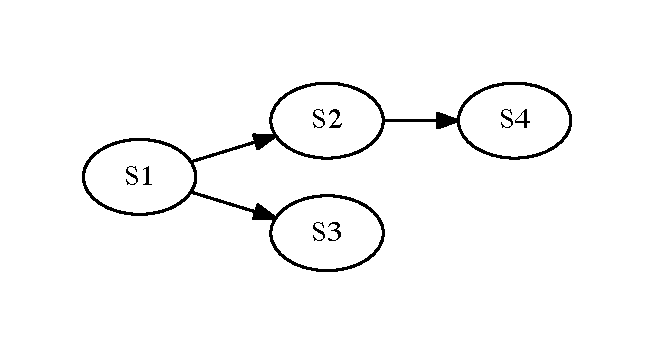
\includegraphics[width=4cm]{graphs/exemple1}}
\caption{ An Example of abstract services precedence graph. }
\end{figure}
\end{example}

Each abstract service may be realized by several concrete services. When abstract service orchestration is defined, we need to choose an appropriate concrete service that performs each corresponding service. Services composition can be seen as a workflow where activities and tasks can be carried out by users and machines in an IoT environment. %The workflow describes how activities or tasks should be carried out. 
In this paper, the possible concrete services organization in order to realise an end-to-end user service according to  a given abstract service orchestration is denoted by concrete workflow. Figure~\ref{figureConcreteOrchestration} gives an example of concrete workflow for orchestration given in figure \ref{figureOrchestration}.

\begin{figure}[htpb]
\label{figureConcreteOrchestration}
\centering \fbox{ 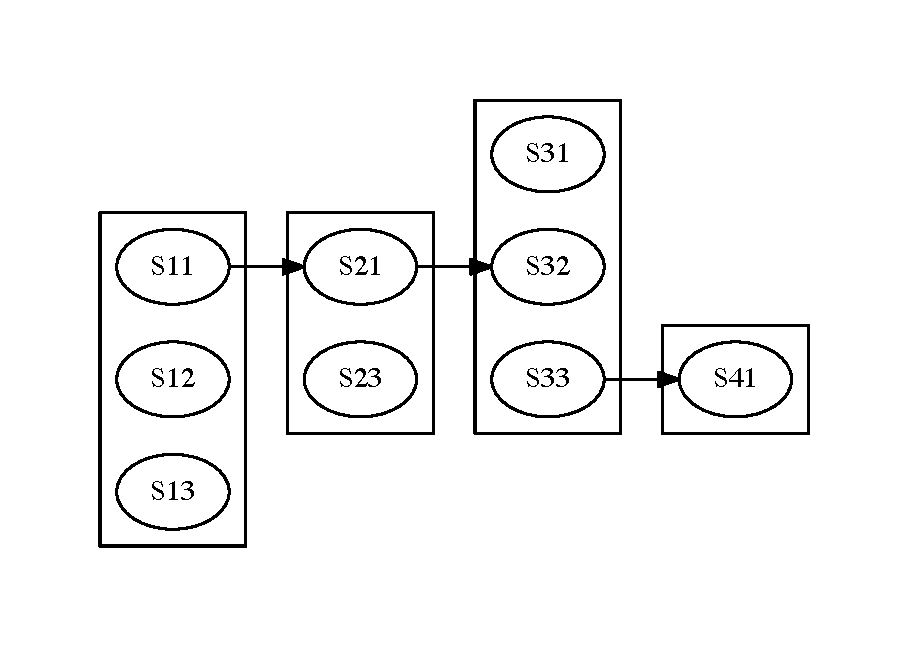
\includegraphics[width=5cm]{graphs/exemple2}}
\caption{ The concrete workflow $(S_{11},S_{21},S_{32},S_{41})$ is a possible organization to realize the orchestration given in figure \ref{figureOrchestration}. }
\end{figure}

Let $f$ be a global objective function that optimizes the end-to-end $Q$ criteria of a service by taking into account some fixed constraints. Let us consider $\psi(S)$ be the $M$ possible abstract service orchestrations in which we denote the $k$-th possible orchestration as $\psi_k$ (for $k\in\{1..M\})$. Thus, $F_{\psi_k}$ indicates the evaluation function of all possible concrete service concatenation of $\psi_k$.%dans le cas ou les services abstrait sont independent, le cout du critère global s'obtient par l'addition des critère de chaque service abstrait

To obtain $F_{\psi_k}$ (For each $k\in\{1..M\}$), it is necessary to select the best concrete service concatenation according to the $Q$ criteria among the concrete services in the given $\psi_k$ orchestration. $\psi_k$  is defined according to the predefined optimisation function $\varphi_{ki,(k \in\{1, \dots,M\}, i \in\{1,\dots,n_k\}}$ on the $Q$ criteria. In our context the $\psi_k$ function will be assumed as linear combination of $Q$ attributes (see example~\ref{ex:linearComb})
 % dans le cas ou la concatenation des services abstrait n'a pas d'impact sur les critères des services concrets l'évaluation de chaque service abstrait ne dépend pas de l'orchestration donc cette étape est inutile 

Without loss of generality, the service selection problem can be defined as follow: find the evaluation function $f$ as the best value of $F_{\psi_k} $


\begin{example}\label{ex:linearComb} Let us consider a problem with three abstract services $\{S_1,S_2,S_3\}$. This problem has a single possible orchestration $\psi(S_i)_{I\in\{1..3\}}=\psi_1$, such that $\psi_1$ represents a serial $(S_1,S_2,S_3)$ orchestration (we execute first concrete services of $S_1$, then $S_2$ and end with $S_3$). Let us consider a problem with two evaluation criteria $Q=\{q_1,q_2\}$, for instance, throughput and service time response. An the concrete services evaluation function (to be optimized later) is defined as a linear combination between these criteria: $\varphi(q_1,q_2)= w_{i1}.q_1+w_{i2}.q_2$ for each abstract service $S_i$. \\
In this case, the problem can be summarized as finding an appropriate weighted parameters $w_{ij}$ by solving the following maximization problem:
$$ \text{max }(\sum_{i=1}^{i=3} w_{i1}.q_1+w_{i2}.q_2)$$
\end{example}

 
%Additional sub-problems must be solved before optimizing the previous problem among which: how to solve the service composition problem without any knowledge about user preferences criteria. 
As explained in the related work section, several studies are done using various approaches. However, some additional constraints make this problem more difficult. The main constraint concerns the fact that no system user preferences are given on the evaluation function components. In this paper, we propose an approach based on discrete time vector valued MDP to estimate the QoS criteria weights respecting the users' preferences for any abstract service orchestration. 

%We propose to learn user preferences from data by using an approach based on discrete time vector valued MDP especially to estimate QoS criteria weights for any abstract service orchestration without requiring user QoS preferences.\\

\subsection{The global problem complexity}
Without loss of generality, let us consider a service composition problem with $n$ abstract services $S_1,\dots, S_n$, such that each abstract service $S_i$ can be concretized by exactly $m$ possible concrete services and there is no explicit constraint between concrete services. The purpose of this section is to enumerate the number of end-to-end concrete service combination in order to evaluate the quality of service of each combination and then to select the best one according to given user or computed preferences.

To the best of our knowledge, there is no existing work dealing with this enumeration problem to evaluate service composition complexity. The main idea of this enumeration is first to evaluate the worst complexity case and then to find a best way to reduce the quality of service evaluation time cost by performing evaluations by equivalence groups for example.  We will present some typical  cases for which we have an exact enumeration and we will give a lower bound for the general case.

\subsubsection{Complexity when there exist a total order between abstract services}
Let us consider $S_1,\dots, S_n$ this order.  Since that each $S_i$ can be realized by $m$ possible concrete services, the possible number of realizations for each order is $n^m$. If there is no additional constraint between abstract services, the number of abstract services permutations will be $n!$. Therefor the  number of  concrete services realizations will be $n!*n^m$.

\subsubsection{Complexity when all abstract services are realized in parallel}
In this case there exists only one possible combination between abstract services. For this alone combination, there exists  $n^m$ possibles realizations. 

\subsubsection{Only two abstract services are realized in parallel}
Let us consider $i$ the number of abstract services realized in parallel and $St(n,i)%=\frac{1}{i!}\sum_{j=0}^{j=i}(-1)^j \binom i j (i-j)^n 
$ the Stirling number of the second kind\footnote{$St(n,i)$ count the number of ways to partition an n-element set into i equivalence classes. It satisfy the recursion formula: $S(n,i)= S(n-1,i-1)+i*S(n-1,i)$.}. \\
If we consider the case where there is two and only two abstract services realized in parallel for a given one total order configuration of abstract services, the number of equivalent classes of length $(n-1)$ is given by $S(n,2)=2^{n-1}-1$. %\frac{1}{2!}\sum_{j=0}^{j=2}(-1)^j \binom 2 j (2-j)^n
 Therefor the number of abstract service configurations will be $(2^{n-1}-1)*(n-1)!$. In this particular case, for each abstract service configuration there is at most $2*(n-1)^m$ possible realizations. We conclude that the possible number of configurations is $2*(n-1)^m*(2^{n-1}-1)*(n-1)!$.

\subsubsection{The complexity in the case of $k$ equivalent classes}
The number of abstract services equivalent classes if given by $S(n,k)$. The number of abstract service configurations will be $S(n,k)*k!$. \\
Let us denote by $CSC$, the number of concrete services configurations and $CSC_k$ the number of concrete service configuration with $k$ equivalent classes.  In this case it is possible to compute upper and lower bound of possible configurations as follow: In all cases, the cardinal of all set of equivalent classes of abstract services is greater or equal to $m$ and for the case of $k$ equivalent classes the set greatest cardinal is $(n-k+1)$. Thereby, it's possible to give the follow bounded result: $m^k*S(n,k)*k! \leq CSC_k \leq ((n-k+1)*m)^k*S(n,k)*k! $

From all that, it is possible to bound the realization number in general case as follow:
$  \sum_{i=1}^{i=n}  (m^i*S(n,i) *i! ) \leq CSC \leq  \sum_{i=1}^{i=n}  (((n-i+1)*m)^i*S(n,i)*i!)$.

$$\ CSC \geq \sum_{i=1}^{i=n}  (m^i*\sum_{j=0}^{j=i}(-1)^j \binom i j (i-j)^n)$$
$$CSC \leq  \sum_{i=1}^{i=n}  (((n-i+1)*m)^i*\sum_{j=0}^{j=i}(-1)^j \binom i j (i-j)^n) $$
% les bornes sont larges, elles peuvent être améliorer. pour une classe d'équivalence l'ordre de grandeur du débordement de la borne par rapport à la valeur exact est  de l'ordre de (n-k-1)^k 

%permutation complete avec égalité : un seul groupe, tous les groupes possibles.
% add some complexity results : maybe use Stirling number of the second kind
% le nombre d'orchestrations serait de n! Si pas de superposition d'états. Ici rechercher la complexité dans le cas ou les états peuvent se superposer. 

\section{Services composition as an MDP problem} \label{sec:Scomp-Formulation}
Markov Decision Processes (MDPs) are the suitable models for sequential decision problems such as QoS decomposition problems. In this section, we describe how to use MDPs to formalize and solve the services composition problem. We are looking for an optimal QoS-selection strategy satisfying the user's requirements in terms of QoS. 
Since the user's preferences with respect to QoS criteria are unknown, %the problem is thus considered as a multi-objective service composition under uncertainties. Accordingly, 
we use a partially known MDP model and more particularly a Vector-valued MDP (VMDP) model. Before getting into details, it is required to describe some preliminary properties and definitions.\\

\begin{definition}
A \textbf{concrete service} $S_{ij}$, or a concrete service executed by an actor with or without time reference properties can be described by several \textit{functional} and \textit{non-functional} properties.

\begin{itemize}
\item Functional properties are generally described under the form of transaction function namely Action$(S_{ij})$ that takes an input data vector InputData$(S_{ij})$ to produce an output data vector OutputData$(S_{ij})$
\item Non-functional properties are including a vector of QoS attributes $Q(S_{ij})$, a set of quality of experience criteria (QoE), and other aspects about the service such as energy consumption and the context of use.  
\end{itemize}
\end{definition}

\begin{definition}
An \textbf{abstract service} $S_i = \{ S_{i1}, \cdots, S_{in_i} \}$ is a class of $n_i$ concrete services with similar functional properties. That means they have the same input data vector and output data vector, but their non-functional properties are different.\\
\end{definition}

In the rest of this section, we will explain how various classes of abstract services, each one including many concrete services can be modeled as a Vector-valued MDP. 

\subsection{Vector-valued Markov Decision Process}
Referring to Section~\ref{sec:problem-formulation} invoking each concert service in a time step $t$ produces different quality of services. In Example~\ref{example:DB}, invoking concrete service $3104$ for abstract service $19994$ at time $5$ gives two different values $0.238$ and $0.733$ for the response time and throughput respectively: $Q(S_{ij}) = (\text{rt}(S_{ij}), \text{tp}(S_{ij}))$. \\

\begin{definition}
Formally, a \emph{Discrete-time Markov Decision Process (Discrete-time MDP)} \cite{timeMDP} is defined by a tuple $(T, S, A, P_t(.|s,a), r_t)$ where:

\begin{itemize}
\item[-] $T=0,\cdots, N$ are the decision time steps at which the decisions are made\footnote{time steps can be days, hours, minutes or any time interval}. 
\item[-]States: $S$ is a finite set of states
\item[-] Actions: $A(s)$ is a finite set of actions that agent can select in state $s$.
\item[-] State Transition Probability Distribution: $P_t(s'| s,a)$ encodes the probability of going to state $s'$ when the agent is in state $s$ and chooses action $a$.
\item[-] Reward Function: $r_t : S \times A \longrightarrow \mathbb{R}$ where $r_t(s,a)$ quantifies the utility of performing action $a$ in state $s$ at $t$ time step.
%\item[-] Discount Factor: $\gamma \in [0,1)$ indicates how less important are future rewards in compared to the immediate ones. 
%\item[-] Initial State Distribution: $\beta : S \longrightarrow [0, 1]$ indicates that the probability that the agent starts her interactions with the environment in state $s$ is $\beta(s)$.
\end{itemize}

\end{definition}

A \emph{Decision rule} $d_t$ is a function depending on time $t$ that defines what action $d_t(s) \in A(s)$ at time $t$ the agent should select. By assuming $N$ number of time steps, we define \emph{policy} $\pi = (d_1, \cdots, d_{N-1})$ as a sequence of $N-1$  decision rules. The policy is stationary if the decision rule for all time steps are the same i.e. : $\forall \; t \in \{1, \cdots, T \} \; d_t = d$. 

A solution for an MDP is a policy $\pi: S \longrightarrow A$ that associates an action to each state. Normally, policies are evaluated by a value function $v^{\pi} : S \longrightarrow \mathbb{R}$. The value function is computed recursively using several recursive functions: %namely \emph{Bellman equations}:
\begin{equation}
v^{\pi}_N(s) = r_N(s, \pi(s)) \;\; \forall s\in S_T
\end{equation}

where $S_T$ is the set of terminal states as a subset of all states. % Remind that there is no action decision in $S_T$ as the set of terminal states. 
For the rest of time steps $t<T$, the value function is defined as:

\begin{equation}\label{eq:value-func}
v^{\pi}_t(s) =  r_t(s,\pi(s)) + \gamma \sum_{s' \in S} P_t(s'|s,\pi(s)) v_{t+1}^{\pi}(s')
\end{equation}

where $\gamma$ is a discount factor and $ 0 < \gamma \leq 1$. Therefore, the preference relation among policies is defined as below:

\begin{equation}
\pi \succeq \pi' \Leftrightarrow \forall s \in S \; v_0^{\pi}(s) \geq v_0^{\pi'}(s)
\end{equation}

The \textbf{MDP solution} is an \emph{optimal policy} which is the highest policy with respect to the other policies and w.r.t $\succeq$, i.e. $\pi *$ is an optimal policy if $\forall \; \pi, \; \pi^* \succeq \pi$.


To find such a policy/workflow, we can use a dynamic programming, namely \emph{Bellman Equation}. 
\begin{equation}
v_N^* = r_N(s) \; \forall s\in S_T
\end{equation}
%
and for all $t= 1, \cdots, N-1$ and $s \in S$, the value of the optimal policy is computed as:
\begin{equation}\label{eq:bellman}
v_t^*(s) =\text{max}_{a \in A(s)} \left \{ r_t(s,a) + \gamma \sum_{s' \in S} P(s'|s,a) v_{t+1}^*(s') \right \} 
\end{equation}

For the sake of simplicity, we define Q-value function on state $s$ and action $a$ at time step $t$ as:

\begin{equation}
Q_t(s,a) = r_t(s,a) + \gamma \sum_{s' \in S} P(s'|s,a) v_{t+1}^*(s')
\end{equation}
In the other hand, the optimal policy is the policy that selects action $a^*$ at stage $t$ from the following:
\begin{equation}\label{eq:opt-action}
a^*_t \in \text{argmax}_{a \in A(s)} \left \{ Q_t(s,a) \right \} \; \text{ for } t=1 \cdots N-1
\end{equation}

Sometimes, selecting an action in a given state and a given time step may have several effects instead of only one value. Therefore, by extending the discrete-time MDP to a discrete-time vector-valued MDP, we have: \\

\begin{definition} \cite{alizadeh:hal-01358345}
A \textbf{discrete-time Vector-valued MDP (discrete-time VMDP)} is defined by a tuple $ (T, S, A, P_t(.|s,a), \bar{r}_t)$ where the vector-valued reward function $\bar{r}$ is defined on $S \times A$ and $\bar{r}(s, a) = ({r_1}_t(s,a), \cdots, {r_d}_t(s,a)) \in \mathbb{R}^d$ is the vector valued reward defined by $\bar{r}$ in state $s$ and action $a$. 
\end{definition}

Notice that the VMDP is another form of Multi objective MDP. That means, $d$ is the number of objectives in the environment while each element $i$ in reward vector $\bar{r}(s, a)$ indicates cost of the $i$-th objective in the model by selecting action $a$ in state $s$. 


\subsection{Service composition as a discrete-time VMDP}%{MDPs for Service Compositions}
By modeling the service composition as a discrete-time VMDP, we can compute the best selected concrete service composition satisfying user requirements in terms of QoS. We assume that, we are allowed in this work to communicate with users in order to get information about their preferences with respect to QoS criteria. We use discrete-time VMDP modeling to select the optimal concrete service for each abstract service w.r.t time stage $t$. For the sake of simplicity, this model is noted as the discrete-time VMDP-Services Composition (discrete-time VMDP-SC) which is introduced hereafter (see \cite{Wang2010, Mostafa2015}).\\

\begin{definition}
A \textbf{VMDP-Service Composition (VMDP-SC} is a tuple $(T, AS, CS, P_t(.|as,cs), \bar{r}_t, AS_T)$, where  

\begin{itemize}
\item[ -] $T= 1 \cdots N$ is a total number of time stages. 
\item[-] $AS$ is a finite set of abstract services.
\item[-] $CS$ is a set of all concrete services, where $CS(S_i)$ indicates a set of available concrete services for the abstract service $S_i \in AS$.
\item[-] $P_t(S_j | S_i, S_{ik} )$ is the probability of invoking the concrete service $S_{ik}$ for abstract activity $S_i$ and resulting in the abstract activity $S_j$.
\item[-] $ \overline{Q}_t: AS \times CS \longrightarrow \mathbb{R}^d$ is a reward function. The $\overline{Q}(S_i, S_{ik})$ reward is the generated Q vector value after invoking $S_{ik}$ in $S_i$ at time step $t$. Given that $d$ represents the number of QoS criteria, we obtain $\overline{Q}_t(S_i, S_{ik}) = ({q_1}_t(S_i, S_{ik}), \cdots, {q_d}_t(S_i, S_{ik}))$. 
\item[-] $AS_T$ is the set of terminal services. The execution of the service composition terminates in one of these states.
%\item[-] $\beta(sa)$ represents the probability of starting abstract activity in abstract service $sa$. Remind that $\sum_{sa \in SA} \beta(sa) = 1 $. ({\color{red} if I remove $\beta$, I will use the MDP model with start abstract services such as \cite{DBLP:journals/tase/KhanoucheACKY16}. })
\end{itemize}

\label{def:vmdp-sc}
\end{definition}

In fact, the solution for QoS-aware service composition is the optimal policy for VMDP-SC model.

\begin{definition}
A \textbf{policy service composition} $\pi: AS \longrightarrow CS$ is a function that defines which concrete service should be invoked for each abstract service in order to give the best trade-offs among multiple QoS criteria. 
\end{definition}

This policy is known as a workflow or composition in the IoT services composition literature. Since reward values in MDP-SC are the $Q$ vectors for each concrete service, each policy should be evaluated with the following vector function (see Equation~\ref{eq:value-func}):
\begin{equation}
\bar{v}_t^{\pi}(S_i) = \overline{Q}_t(S_i, \pi(S_i)) + \gamma \sum_{S_j \in S} P(S_j | \pi(S_i), S_i) \bar{v}_{t+1}^{\pi}(S_j)
\end{equation}

Thus, comparing two composition/policies boils down to comparing two vectors. The optimal compositions satisfying various users with different preferences on the QoS attributes can be different. Thus, we need a model that presents the user preferences over quality of services attributes. \\

%\begin{example}
%Regarding to example \ref{example:DB}, 
%Another examples that shows the relation between user preferences on the QoS attributes.
%\end{example}

For this reason, the Simple Additive Weighting (SAW) technique \cite{qi2010combining} is used to aggregate the QoS attributes values of services into a single utility value by considering user's preferences expressed as weights. The services selection is then transformed into a single objective optimization problem to find the candidate services providing the best utility value. In fact, if any user gives a  weight to each attribute, the dependency between the users' weights and quality of service attributes is defined as below:

\begin{multline}
Q_t(S_i, S_{ij}) = \sum_{k=1}^d \bar{w}_k {q_k}_t = \bar{w} \cdot \overline{Q}(S_i, S_{ij}) \\
\forall t = 1, \cdots, N
\end{multline}

where $\bar{w} = (w_0, \cdots, w_d) $ is a weight vector, indicating the user preferences on the QoS attributes such that 
\begin{equation*}
\sum_{i=1}^d w_i = 1
\end{equation*}

If user's preferences on QoS attributes are given, the optimal composition can be therefore computed easily using SAW technique. However, determining appropriate weights for QoS attributes needs knowledge of user preferences, which is often not obvious to obtain in practice. Even if user preferences have been obtained, setting accurately these weights remains a problem. For instance, it is hard to decide the weight of response time as 0.2 or 0.21, which appears no big difference yet it can affect the result of the QoS optimal composition \cite{chen2015partial}. Accordingly, we assume that $\bar{w}$ is unknown and try to find the best composition/policy by querying users when it is necessary.\\

To compare workflow vector values with each other, we consider first, the unknown weight vectors are confined in a $d-1$ dimensional polytope $W$ such that:
\begin{equation}
W = \{ (w_1, w_2, \cdots, w_d) \; | \; \sum_{i=2}^d w_i \leq 1 \; \text{and} \; w_1 = 1-\sum_{i=2}^d w_i \}
\end{equation}

To compare Q vector values with each other, we can use three different comparison methods. Assume $\bar{v}^a = (a_1, \cdots, a_d)$  and $\bar{v}^b = (b_1, \cdots, b_d)$ are two $d$-dimensional vectors representing expectation of sum of QoS values for two workflows $a$ and $b$. 

\begin{itemize}
\item[-] the most natural comparison method is \emph{pareto comparison} that defines:
\begin{equation} \label{eq:pareto}
\bar{v}^a \succeq_P \bar{v}^b \Leftrightarrow \forall \; i \; a_i \geq b_i
\end{equation}\label{eq:kdom}
\item[-] \emph{Kdominance comparison} defines $\bar{v}^a$ is more preferred than $\bar{v}^b$ if, it is better for any $\bar{w}$ in polytope $W$:
\begin{equation}
\bar{v}^a \succeq_K \bar{v}^b \Leftrightarrow \forall \; \bar{W} \in W \; \bar{W} \cdot \bar{v}^a \geq \bar{W} \cdot \bar{v}^b
\end{equation}\label{eq:queryuser}
\item[-] query this comparison to the user, i.e. $\bar{v}^a  \succeq_q \bar{v}^b$. 
\end{itemize} 

We remind that, the Kdominance comparison is a linear programming problem. In other words, $\bar{v}^a  \succeq_K \bar{v}^b$ is satisfied if there is a non-negative solution to the following LP:
\begin{equation}
\left\{
\begin{array}{ll}
\text{min} \; \bar{W} \cdot (\bar{v}^a - \bar{v}^b) \\
\text{subject to } \; \bar{W} \in W
\end{array}
\right.
\end{equation}
If there is no non-negative solution for two comparisons $\bar{v}^a  \succeq_K \bar{v}^b$ and $\bar{v}^b  \succeq_K \bar{v}^a$, these two vectors are not comparable using the Kdominance. \\

In the rest of this paper, we will explain how to find the optimal composition/policy that gives the best trade-off among multiple QoS criteria, satisfying the user requirements in terms of QoS by querying him very few times. % Since we are interested in computing the best match for each agent regarding her preferences, our algorithms queries the agent when it is required. %Therefore, the proposed queries to the agent get the partial information on their preferences on the QoS attributes.  

\section{Interactive Reinforcement Learning Algorithms for the Service Compositions}  \label{sec:Inter-Alg}
We propose an algorithm namely \emph{Interactive Value Iteration for Service Composition (IVI-SC)}. Previously, we explained how model the services composition problem as a discrete-time MDP. In this section, we describe how to find the solution using the existed solutions for MDPs. Some researchers use interactive value iteration methods to find the optimal policy respecting the user of system preferences \cite{weng:hal-00942290,alizadeh:hal-01358345}. In this paper, we modified the interactive value iteration on a finite-horizontal MDP to find the best service composition satisfying users' requirements in terms of QoS. We assume that an MDP model of services (VMDP-SC) with finite discrete-time is given. The services can be invoked in $T+1$ number of discrete time steps: $\{0, \cdots,T-1 \} \cup \{T\}$ where $T$ is a final empty time stage. %That means, the quality of all the invoked concrete services in time step $T$ are zero.
Since the MDP-SC objective is finding the policy that maximizes a measure of long-run expected Q vectors, we propose a backward induction method to solve the Bellman equation given in equation~\ref{eq:bellman} and finds the optimal actions given in equation~\ref{eq:opt-action} to obtain the optimal policy/work-flow. Our solution is introduced in Algorithm~\ref{algo:ivi}.

\begin{algorithm}[]
\label{algo:ivi}
 \KwData{VMDP-SC$(T, AS, CS(), P_t, \bar{r}_t)$, a $W$ polytope of user weights on objectives}%, precision $\epsilon$}
 \KwResult{The optimal service selection policy for the given user. }
 $t \longleftarrow T$ \\
 $\pi_{\text{best}} \longleftarrow $ choose random policy \\
$\bar{v}_{T}(s_T) \longleftarrow (0, \cdots,0)$\footnote{zero vector of dimension $d$ where $d$ is the number of quality attributes for QoS}  $\forall s_T$ at time $T$  \\
 $\mathcal{K} \longleftarrow $ set of constraints on $W$ \\
 \While{$t \geq 0$}{
 	$t \longleftarrow t-1$ \\
	%\For{\textbf{each} $as \in AS$}{
	\For{$S_{i}(t)$}{%{\textbf{each} $h_t = (h_{t-1}, S_{kj}(t-1), S_{i}(t)) \in H_t$}{
		best $\longleftarrow (0, \cdots, 0)$ \\
		%\For{\textbf{each} $cs_{t-1} \in A(as)$}
		\For{\textbf{ each } $S_{ij}(t) \in CS(S_{i}(t))$}{
			\small{$\bar{v}_t(S_{i}(t)) \longleftarrow \overline{QoS}(S_{i}(t), S_{ij}(t)) + \sum_{S_{m}(t+1)} P_t(S_{m}(t+1) | S_{i}(t), S_{ij}(t)) \bar{v}_{t+1}(S_{m}(t+1))$}\\
			$($ best $, \mathcal{K} ) \longleftarrow $ getBest(best, $\bar{v}_t, \mathcal{K}$) \\
		   	$\bar{v}_t(S_{i}(t)) \longleftarrow $ best \\
		   	\If{best = $\bar{v}_t(S_{i}(t))$}{
				$\pi_{\text{best}(S_{i}(t)) \longleftarrow S_{ij}(t)}$
			}
	 }
	}
 } 
 \textbf{return} $\pi_{\text{best}}$ \\
 \vspace{0.3cm}
 \caption{\textbf{Interactive Value Iteration for Service Composition:} How to select the best composite for each abstract service respecting user preferences on QoS attributes}
\end{algorithm}
%%%%%%%%%%%%%%%%%

%%%%%%%%%%%%%%%%%%%%

\begin{algorithm}[]

\KwData{finds the more preferred vector between two vectors $\bar{v}$ and $\bar{v}'$ w.r.t $ \mathcal{K}$}
\KwResult{}

\If{paretodominates($\bar{v}, \bar{v}'$)}{
	\textbf{return} $(\bar{v}, \mathcal{K})$
}
\If{paretodominates($\bar{v}', \bar{v}$)}{
	\textbf{return} $(\bar{v}', \mathcal{K})$
}
\If{Kdominates($\bar{v}, \bar{v}',  \mathcal{K}$)}{
	\textbf{return} $(\bar{v}, \mathcal{K})$
}
\If{Kdominates($\bar{v}', \bar{v},  \mathcal{K}$)}{
	\textbf{return} $(\bar{v}', \mathcal{K})$
}
$(\bar{v}_{\text{best}}, \mathcal{K}) \longleftarrow $ query$(\bar{v}, \bar{v}',  \mathcal{K})$ \\
\textbf{return} $(\bar{v}_{\text{best}}, \mathcal{K})$
\caption{\textbf{Best}: this algorithm finds the most preferred vector between two given vectors.}
\end{algorithm}\label{algo:getBest}
%%%%%%%%%%%%%%%%%%%%

In the iterative algorithm~\ref{algo:ivi}, first we assign a zero vector to the set of states (abstract services) at time step $T$. For each abstract service $S_i(t)$ (in time $t$) given in the MDP-CS, the algorithm selects the best concert service among the all available ones. These actions (concrete services) are dependent on various time steps, for instance the possible actions of the $S_i(t)$ service in times step $t$ can be different from the possible actions for time step $t+1$. In the finite horizon time (our case), the iteration continues until either this difference becomes small enough or the horizon time steps finish. 

%%%%%%%%%%%%%%%%%%%%
\begin{algorithm}[]
\KwData{$\bar{v}, \bar{v}', \mathcal{K}$}
\KwResult{ it queries the comparison between $\bar{v}$ and $\bar{v}',$ to the user and modifies $\mathcal{K}$ according to her response.}
Build query $q$ for the comparison between $\bar{v}$ and $\bar{v}'$ \\
\If{if the user prefers $\bar{v}$ to $\bar{v}'$}{
	\textbf{return} $(\bar{v}, \{ (\bar{v} - \bar{v}') \cdot \bar{W} \geq 0 \})$
}
\Else{
	\textbf{return} $(\bar{v}', \{ (\bar{v}' - \bar{v}) \cdot \bar{W} \geq 0 \})$
}
\caption{\textbf{query}: queries the user about her preferences on existed quality of services.}
\end{algorithm}\label{algo:query}

Since the quality of services are the $d$ dimensional vectors, solving equation~\ref{eq:bellman} and finding the maximum among the vectors is not obvious. For this reason, we remind three comparison methods (presented in equations~\ref{eq:pareto}, $13$ and $14$ %~\ref{eq:kdom} and~\ref{eq:queryuser}
) and utilize the \textbf{Best} function (given in Algorithm~\ref{algo:getBest}). This function receives two $d$ dimensional vectors with the $W$ polytope confining the user weight preferences on the quality of services. If the pareto comparison can not find the greater vector, we will test the Kdominance comparison for finding the most preferred vectors. Otherwise the query function should be called (given in Algorithm~\ref{algo:query}). The user's response to the comparison between the two given vectors, adds a new constraint to the $W$ polytope. 

Algorithm~\ref{algo:ivi} finally finds the optimal policy/work-flow or service composition for the given system MDP-SC and returns back the optimal policy $\pi_{\text{best}}$. Notice that the condition $best = \bar{v}_t(S_i(t))$ in Algorithm~\ref{algo:ivi} checks if the best selected concrete service for $S_i(t)$ has been changed regarding the previous iteration. If it is, the optimal concrete service should be replaced by the concrete service $S_{ij}(t)$ which generates a better vector value for $S_i(t)$. 
 
%\section{Time complexity analysis} \label{sec:complex-analys}
The complexity of the proposed algorithm as an exact algorithm is polynomial w.r.t three parameters : 1) the number of abstract services forming the composition, the number of candidate services per each abstract services, and the number of QoS criteria. Assume $|AS|$ is the set of all abstract services and $M = \text{max}_{i,t} CS(S_i(t))$ is the maximum number of abstract services in each time step $t$ and each abstract service $S_i$. %For designing the MDP-CS, we take all users execution observations into account. Then each concrete service $S_{ij}$ adds maximum up to number of users to the actions.
For computing the best QoS vector in each inner iteration, the \textit{Best} algorithm tests the pareto dominance and k-dominance comparison twice in the worst case which are polynomial w.r.t $d$. $d$ is the number of attributes for quality of services and any k-dominance (LP) can be solve in polynomial time. Then, the algorithm has $O(T.|AS|.M.d)$ where $T$ is the number of time stages. 

\section{Performance Evaluation}\label{sec:results}


\cite{mostafa2015multi} introduces a method for finding the list of all non-dominated service composition regardless of user weight preferences $\bar{W}$ on QoS attributes. That means, each exact computed service composition is included in this set. For this reason, IVI-SC proposes an algorithm for computing the exact service composition for each system user. In the following we show how the experimental results work. 

We evaluate our methods on a public available data-set containing two parameters for quality of services: throughput and response time. These are the records between $339$ users and $5825$ web services distributed worldwide \cite{Zheng2014,Zheng2015}. The data-set also includes some information about user features and service features such as countries, autonomous systems, IP dresses, latitude and longitude. In the studied data base, $142$ users execute various web services in different time slices. Practically, the information are given only for $64$ time steps. In this section, we first explain how to model the dataset as a VMDP-SC and then we will examine our algorithm on the data-set. 

\subsection{Data-Set as a VMDP}
The main issue in implementing IVI-SC (Algorithm~\ref{algo:ivi}) on any database is that how to model the given data-set as a vector-valued MDP. In the supported dataset \cite{Zheng2014,Zheng2015}, there are several text files including wslist.txt, userlist.txt, rtdata.txt and tpdata.txt. The wslist.txt represents some information on various web services and their related abstract services. It is our source file for extracting a list of web services and their related abstract services; if a related abstract service exists for the selected web service. The userlist.txt includes some information about users of different web services. The two other files tpdata.txt and rtdata.txt include the throughout and response time values respectively on various web-services executed by $142$ users. That means any invoked web service by a user has two parameters for measuring the service quality: throughout and response time. 

\begin{figure}[t]
\label{fig:seq-mdp}
\centering
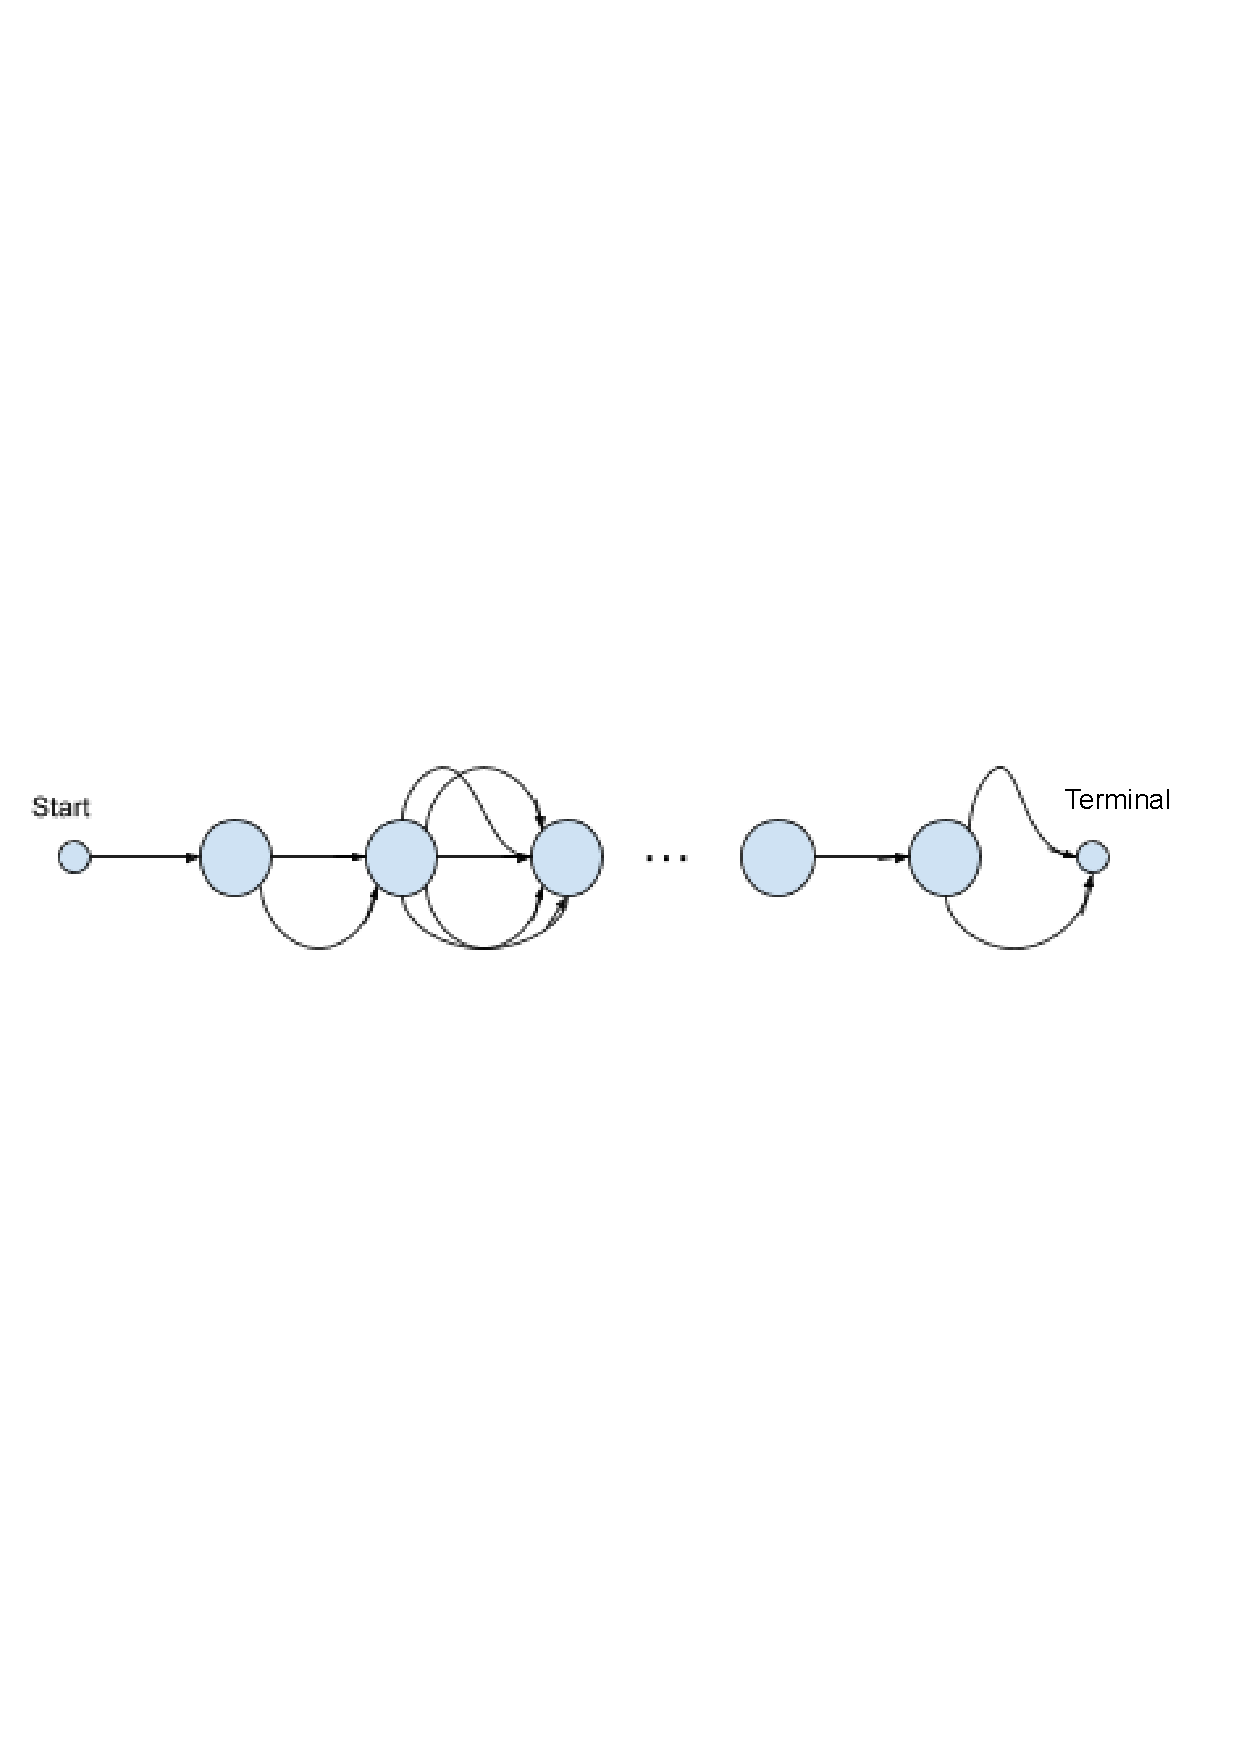
\includegraphics[width=9cm]{graphs/seq-mdp-}
\caption{A sequential form of abstract service connection}
\end{figure}

The studied database\cite{Zheng2014,Zheng2015} is generated in real by observing various users utilizing enormous number of web services. We notice that all provided data inside database are not useful. After extracting all web services and their related abstract services from wslist.tx file, and getting the web services qualities from two files tp.txt and rt.txt, we have a VMDP-SC with the following parameters (refer to~\ref{def:vmdp-sc}) :
\begin{itemize}
\item[-] number of episodes:  $N=64$
\item[-] $744$ number of abstract services 
\item[-] $3551$ total number of concrete services (in our case web services)
\item[-] The transition function and terminal states depend on the proposed model or relation types among the abstract services. 
\item[-] and the $\overline{Q}_t$ function is built based on the extracted data on web services and their two qualities (response time and throughout).
\end{itemize}

To demonstrate the efficiency of our approach in calculating the optimal workflow, we study our method on a common model in state of the art: the sequential model. %and parallel model. 

%\begin{itemize}
%\item[1] 
For the sequential model (see Fig~\ref{fig:seq-mdp}) the start sate is an empty state and connected to the first selected abstract service in the model. On the other hand, the terminal state is an empty state that indicates the MDP is a finite horizon one. In this model, the sequential order on abstract services can be defined in any order. In our model, the order has been selected randomly once to fix the MDP model. For any time step $t \in \{ 0 \cdots 63 \}$, the transition probability $P_t(S_j(t+1) | S_i(t), S_{ik}(t))$ is $1$, if web service $S_{ik}$ is invocable for a given abstract service $S_{i}(t)$ according to our database and abstract service $S_j(t+1)$ is the next demanded service in our selected sequential MDP model, otherwise $P_t(S_j(t+1)| S_i(t), S_{ik}(t)) = 0$. 

%\item[2] For the parallel model (see Fig~\ref{fig:par-mdp}), the start and terminal states are again two empty states. The start state is connected to all abstract services such that $P_t(S_i | S_{\text{start}}, S_{ik}) = \frac{1}{744}$\footnote{$"744"$ is the total number of abstract services of the model. That means each abstract service can be selected in start state. }.  Each state (abstract service) $S_i$ is connected to the terminal state with $|CS(S_i)|$ number of invocable web services for state $S_i$. For all time step $t = 0, \cdots, 63$, $P_t(S_{\text{terminal}} | S_i, S_{ik})$ is $1$ if $S_{ik} \in CS(S_i)$, otherwise it is $0$ . 

%\end{itemize}

\subsection{Model Whole Dataset as VMDP}

\begin{table}
\begin{tabular}{ l | l | }
  user & weight vector \\
  \toprule
   $\bar{W}_0$ & $[0.319797998295 \;\;\;\;\;\;\;\;, \;\;\;\;\;\;\;\; 0.680202001705]$ \\
   $\bar{W}_1$ & $[0.8573741847324399 , 0.14262581526756013]$ \\
   $\bar{W}_2$ & $[0.1696287781131175\;,\; 0.8303712218868825]$ \\
   $\bar{W}_3$ & $[0.6451844883834318\;,\; 0.3548155116165682]$\\
   $\bar{W}_4$ & $[0.47245438345\;\;\;\;\;\;\;\;\;\; , \;\;\;\;\;\;\;\;\;\; 0.52754561655]$\\ 
 \end{tabular} 
 \caption{The weight vectors for $5$ system users with various preferences on the attributes (throughput, response time).} 
 \label{table:weights}
\end{table}

To evaluate algorithm~\ref{algo:ivi} on our supported dataset, we consider the complete dataset. That means, we keep all quality services executed by all $142$ users. Modelling the huge size data base as a VMDP-SC and implementing the IVI-SC (\ref{algo:ivi}) on the model is challenging.  

\begin{figure}[t]
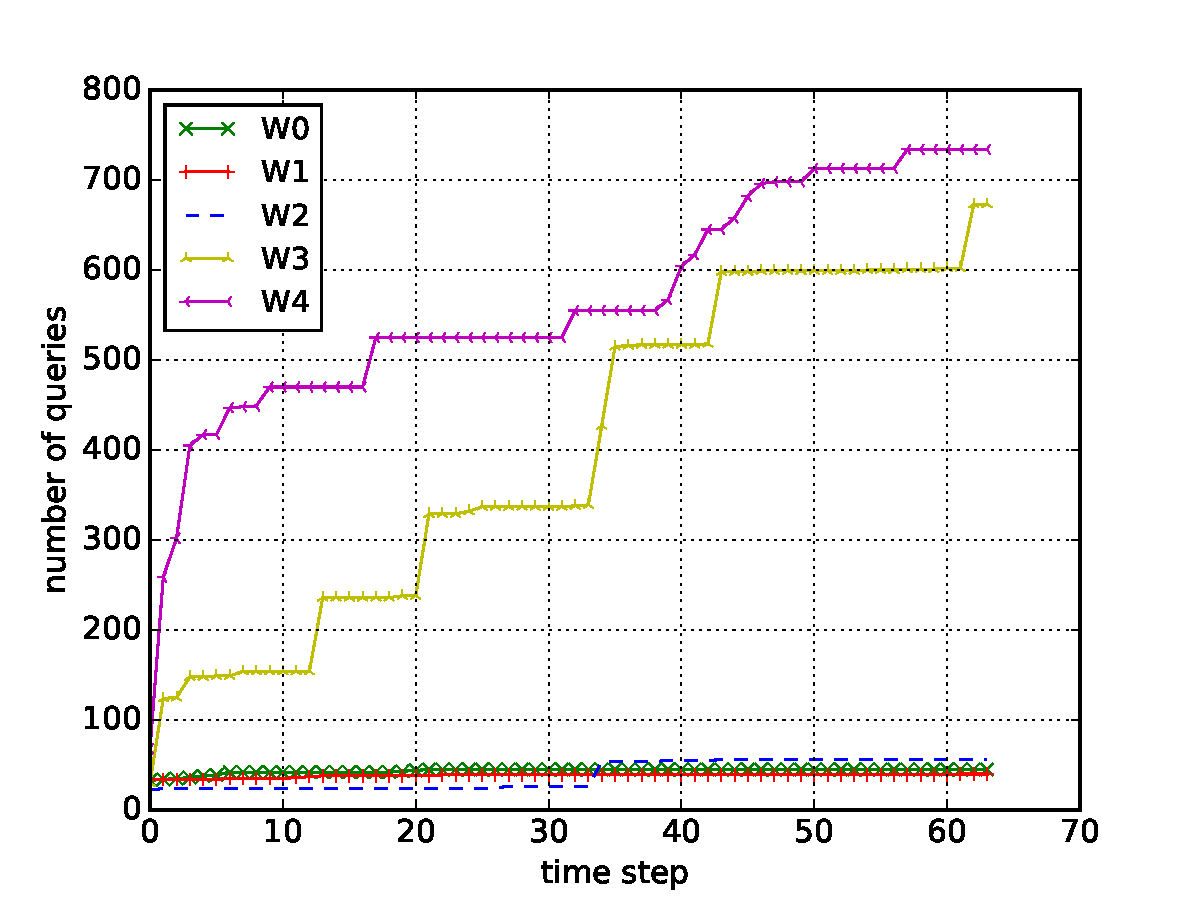
\includegraphics[width=8cm]{new_graphs/time-queries-all++.pdf}
\caption{This figure shows the number of queries proposed to the user during each time step. The weight preferences are based on table~\ref{table:weights}.}
\centering
\label{fig:queries-vs-timestep}
\end{figure}

In order to evaluate our algorithms performance, we analysed the results for $5$ different users systems with various preferences on the service qualities: response time and throughput. Our tested user weights vector ($\bar{W}$) on service qualities is given in table~\ref{table:weights}. Notice that the weight preferences on quality of services are "unknown`` to our algorithms. Our proposed algorithm~\ref{algo:ivi} calculates the optimal workflow while learning the users weight preferences on the attributes. We mention the weight vectors for the simplicity of demonstrating the experimental results and to compare them with the learned weights from Algorithm~\ref{algo:ivi}.

\begin{table}[ht]
\caption{This table demonstrates how each predicted service composition from algorithm \ref{algo:ivi} is different from the exact service composition for $W_2$.}
\centering
\resizebox{\columnwidth}{!}{%
\begin{tabular}{lc|cc||cc||cc}
%\hline
% & &  \multicolumn{2}{c||}{} & \multicolumn{2}{c||}{}\\
\hline
Services & \shortstack{ \tiny{number} \\ \tiny{of WS}} &IVI& Exact & Services & \shortstack{ \tiny{number} \\ \tiny{of WS}}& IVI & Exact  \\
\hline
AS14280& 2& 566 & 567 &   
AS9829& 2 & 1559 & 1565 \\
AS6360& 3 &3723 & 3725 &
AS29650 & 2 &1583 & 1586\\
AS4766& 9 & 2226 & 2237 & 
AS4768&2 &2053 &2054\\
AS3288  & 2& 1622&1623 & 
AS42695&2 & 2503& 2504\\
AS20284 &8 &1547& 1554 & 
AS42915& 3&1588 &1590 \\
AS852&7 &533 &4126 &
AS22047& 2&612 &613 \\
AS14415& 13&4120& 4119 &
AS50517& 3&2304& 2306 \\
AS16265&2 &2018& 2665 & 
AS5050& 4&3584 &3586 \\
AS13301& 6&1382& 1487 & 
AS13041& 24&2375& 2368 \\
AS15806&7 &1566 &1576 &
AS47720& 3&1569& 1571\\
AS11955& 12&3882 &3888& 
AS8075& 11&12 &4183\\
AS33821& 2&2256& 2258& 
AS23148& 5&583 &4233\\
AS29944 & 3&4223& 4224& 
AS35041 &2 &2514 &2533\\
AS20773 & 6&1348& 2548&
AS6830 &2 &1579 &1584\\
AS17819 &4 &2325 &2329& 
AS7050 & 4&4198 &4201\\
AS27437 & 3& 4047& 4050& 
AS48347 & 3&2271 &2273\\
AS19855 & 3&3652 &3653&
AS760& 3& 90 &92\\
AS23650 & 22&625& 853& 
AS8737 & 13&1932 &1940\\
AS87 & 5&4111 &4112& 
AS9116 &2&1615& 1630\\
AS8551 & 4&1620 &1634& 
AS19875& 5& 547& 549\\
AS15366 & 4&1244& 1246& 
AS55481 & 4&44 &47\\
AS5603 & 2&2345 &2349&
AS39418 &10 &959 &970\\
AS31727 & 4&1582& 2922& 
AS5786 & 3&2212 &2214\\
AS9848 & 4&2232 &2233& 
AS29097 & 3&2538& 2540\\
AS29076 &5 &2275 &2293& 
AS29951 & 8&3856& 3860\\
AS4808&10 & 670& 770&
AS32577 & 10&3640 &3638\\
AS17431& 2& 752 &753& 
AS32475& 3& 3728& 3729\\
AS2819& 5& 918 &946& 
AS3786 & 13&2215& 2225\\
AS32613 &3 &93 &94& 
AS27030 & 3&4467& 4469 \\
AS11305 & 3&3688 &4046& 
AS24969 & 2&999 &1004\\
AS15670 & 3&1982 &1984& 
AS1251 & 10&175 &194\\
AS156 & 2&4179& 4180& 
AS12714&2 & 2279& 2280\\
AS16095 &3 &998 &1016& 
AS16245 & 2&1000 &1018\\
AS15290 & 6&536 &574&
AS8542& 6& 2081& 2090\\
AS31815 &11 &4236& 4414&
AS34235 & 4&1141 &1208\\
AS8151 & 3&1918 &1919&
AS9308 & 5&748 &801\\
AS4812 & 11&760 &862& 
AS5409 & 2&1440& 1441\\
AS3389& 4& 4109 &4106&
AS8928& 2& 1202 &3045\\
AS81&5 & 509& 510&
AS3561 &25 &3647& 3579\\
AS6785 & 2&955 &956& 
AS8659 & 4&2543 &2545\\
AS45061 & 12&648 &649& 
AS44249& 10& 2171& 2173\\
AS702& 16& 156 &1147 &
AS701 & 19&3493 &3491\\
AS22070 & 2&3661& 3662& 
AS11426&50 & 3207 &3163 \\
AS1128 & 5&1964 &1965& 
AS2611 &10 &132 &140\\
AS25518& 2& 1774& 1775&
AS14584 & 4&3894 &3896 \\
AS224&7 & 2115 &2075&
AS16339& 2& 2911& 2912\\
AS15348& 3& 3731 &3732&
AS16237 &4 &1959 &1960\\
AS31827& 3& 4341 &4342&
AS32&9 & 4387 &4388\\
AS30190& 2& 4408 &4409&
AS9143 & 8&1974 &1991\\
AS8220 & 15&160& 1182&
AS9318 & 6&2229& 2243 \\
AS4230 & 8&167& 199&
AS22489 & 3&210& 211\\
AS43200& 3& 2087& 2089&
AS3307 & 3&2091 &2120\\
AS3301& 6& 2506 &2522&
AS9811 & 3&695 &697\\
AS34779& 9& 2332 &2335&
AS73& 4& 3911 &3914\\
AS553 &2 &1448 &1466& 
AS12859&7 & 125 &2024\\
AS15756& 3& 2283 &2298&
AS15879& 4& 1961 &2029\\
AS10929& 4& 4065& 4066& 
AS15085& 2& 554 &555\\
AS21844& 13& 4163 &4161&
AS12731& 4& 1361 &1378\\
AS237 & 6&3523 &816&
AS195 & 13&4188& 4027\\
AS1226& 3& 4010& 4012& 
AS1221& 2& 43 &79\\
AS8358& 2& 1521& 1522& 
AS680 & 44&1398 &1401\\
AS8&3 & 3667& 3668&
AS3316&4 & 2260 &2261 \\
AS4837 &29 &680 &791&
AS27617& 3& 4445& 4446\\
AS8190& 3& 4067& 4068&
AS8904& 5& 2264 &2266\\
AS43541& 3& 913 &915& 
AS2519& 4& 1857& 1859\\
AS42949& 2& 1994& 1995& 
AS18125& 5& 1861 &1862\\
AS2200 & 28&1120 &1108&
AS26228& 6& 2077 &2080\\
AS19024& 8& 3924 &3929&
AS11343& 3& 4444 &4442\\
AS40142& 7& 3740 &3767&
AS1103 & 3&1989& 1992\\
AS33491& 3&3681& 3682&
AS33494 & 9&3700 &3707\\
AS12695& 3& 2277& 2291&
AS9120 & 2&1011 &1028\\
AS41635& 3& 2250 &2252& 
AS21309 &3 &1792 &1794\\
AS8342 & 5&950 &2269&
AS12306 & 9&736 &4317\\
AS12301 & 3&1512 &1514&
AS9338& 9& 2040 &2046\\
\hline
\end{tabular}
}
\label{table:W2_0}
\end{table}


\begin{table}[ht]
%\caption{This table demonstrates how each predicted policy from algorithm \ref{algo:ivi} is different from the exact optimal workflow for $W_2$.}
\centering
\resizebox{\columnwidth}{!}{%
\begin{tabular}{lc|cc||cc||cc}
%\hline
% & &  \multicolumn{2}{c||}{} & \multicolumn{2}{c||}{}\\
\hline
Services & \shortstack{ \tiny{number} \\ \tiny{of WS}} &IVI& Exact & Services & \shortstack{ \tiny{number} \\ \tiny{of WS}}& IVI & Exact  \\
\hline
AS10694&9 & 4123& 4354&
AS3778 & 7&3839 &3838\\
AS6983 & 50&3214 &3234&
AS43220& 2& 980 &981\\
AS39111& 3& 964 &1319&
AS3614 & 4&3539 &3541\\
AS17477& 9& 18 &2062&
AS29134 & 2&939 &940\\
AS43892 & 2&1532 &1533&
AS14335 &2 &3596 &3597\\
AS8972& 3& 1343 &1344&
AS3292& 36& 2068 &2478\\
AS8803&3 & 2554 &2555&
AS12874& 23& 1711& 1821\\
AS1930 & 2&2204& 2208&
AS210 &13 &3709 &3712\\
AS24958 &3 &947 &948& 
AS15083 & 28& 863 &864\\
AS6400 & 4&1030 &1031& 
AS1205& 4& 108& 111 \\
AS8508& 3& 2168& 2169& 
AS11798& 18& 3822& 3824\\
AS36017 & 3&4473 &4474& 
AS55454 & 3&2031 &2032\\
AS36850 & 4&3655 &3657&
AS40619 & 4&3526 &3525\\
AS16276 &8 &1191& 1201& 
AS5537& 2& 2288 &2295\\
AS13367 & 10&3750& 3738&
AS12312& 4& 1365 &1367\\  
\hline
\end{tabular}
}
\label{table:W2_1}
\end{table}

\begin{table}[ht]
\caption{This table demonstrates how each predicted service composition from algorithm \ref{algo:ivi} is different from the exact service composition for $W_4$.}
\centering
\resizebox{\columnwidth}{!}{%
\begin{tabular}{lc|cc||cc||cc}
%\hline
% & &  \multicolumn{2}{c||}{} & \multicolumn{2}{c||}{}\\
\hline
Services & \shortstack{ \tiny{number} \\ \tiny{of WS}} &IVI& Exact & Services & \shortstack{ \tiny{number} \\ \tiny{of WS}}& IVI & Exact  \\
\hline
AS42695 &2 & 2503& 2504&
AS50517 & 3& 2304& 2306\\
AS16265 & 2&2018& 2665&
AS15806 & 7& 1566 &1576\\
AS8075 & 11&3830& 4183&
AS23148 & 5&583 &4233\\
AS35041 & 2&2514 &2533&
AS48347 & 3&2271 &2273\\
AS760&3 & 90 &92&
AS39418 &10 &963& 970\\
AS4808 & 10& 670 &770&
AS32475 & 3&3728 &3729\\
AS32613 & 13&99 &94&
AS156&2 & 4179& 4180\\
AS25260 &5 &1268& 1270&
AS16245& 2& 1000 &1018\\
AS8542 & 6&2081& 2090&
AS5409 & 2&1440 &1441\\
AS3561 & 25&3647& 3579&
AS2611 & 10&132& 135\\
AS14584 & 4&3894& 3896&
AS16237& 4& 1959 &1960\\
AS10929& 4& 4065 &4066&
AS12731& 4& 1361& 1378\\
AS4837 & 29&739 &791&
AS2519 & 4&1857 &1859\\
AS18125& 5& 1861 &1862&
AS2200 & 28&1120 &1052\\
AS26228& 6& 2077 &2080&
AS41635& 3& 2250& 2252\\
AS21309& 3& 1792& 1794&
AS10694 &9 &4123 &4124\\
AS3778 &7 &3836 &3838&
AS39111 &3 &964& 1319\\
AS3614&4 & 3539 &3541&
AS1930& 2& 2204& 2208\\
AS8508 & 3&2168& 2169&
AS36850& 4& 3656& 3657\\
\hline
\end{tabular}
}
\label{table:W4}
\end{table}

Figure~\ref{fig:queries-vs-timestep} shows how the interactive value iteration algorithm communicates with users during $64$ time steps. Since the user weight preferences are unknown to the algorithm, it is required to query them in the required situations. According to the figure, the algorithm~\ref{algo:ivi} does not ask more than $56$ queries to the users with various preferences weights $\bar{W}_0$, $\bar{W}_1$ and $\bar{W}_2$ on the service qualities. On the other hand,for two weight preferences $\bar{W}_3$ and $\bar{W}_4$, the algorithm queries too many questions to the user. Regarding to the QoS values and these weights, comparing vectors using pareto dominant and K-dominant methods are not informative. Thus, finding the optimal workflow is difficult for the similar weights. Since, IVI-SC is an exact algorithm, the initial sequence of data-set presentation have an important affect on the number of required queries for finding the optimal policy. In our next research, we are interested in observing the number of required queries for finding the optimal service composition w.r.t the dataset presentation form. 
%\red{explain the odd case of $W_3$, $W_4$}
%The number of user interruptions is important because in reality users do not continue communicating with the system if they should answer too many questions.

%%%%%%%%%
\begin{figure}[t]
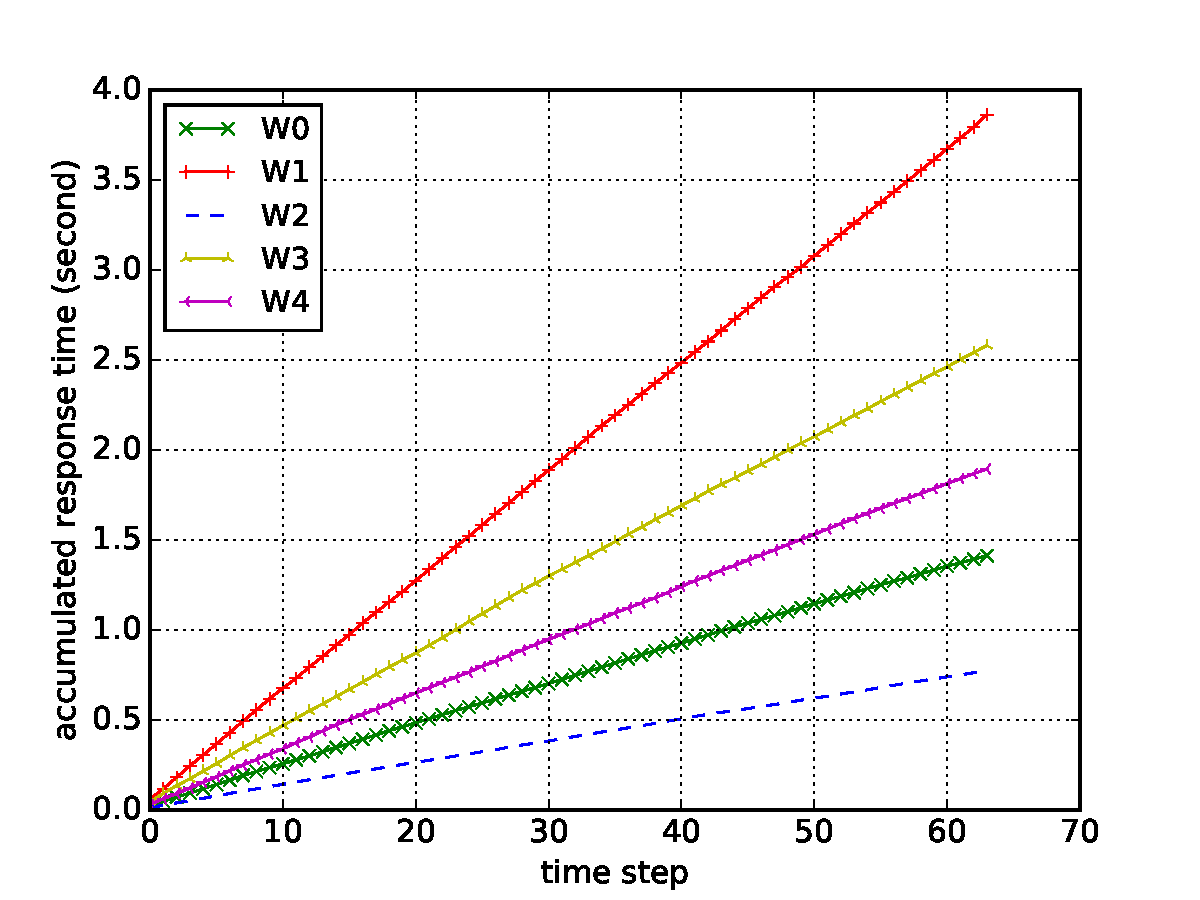
\includegraphics[width=8cm]{new_graphs/rt_step_all++.pdf}
\caption{This figures demonstrate how the accumulated response time increases during each time step. The weight preferences are based on table~\ref{table:weights}.} 
\centering
\label{fig:rt-vs-timestep}
\end{figure}
%%%%%%%

\begin{figure}[t]
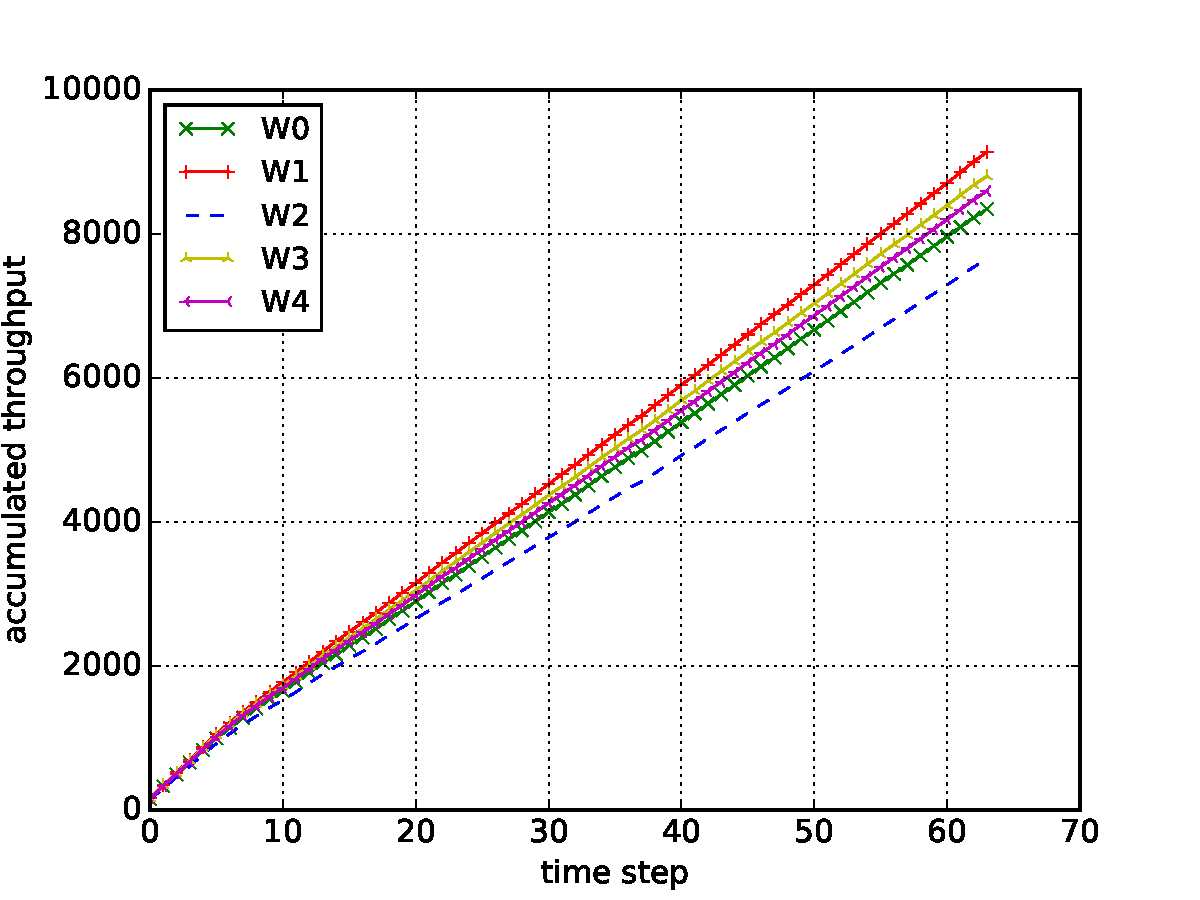
\includegraphics[width=8cm]{new_graphs/trough_step_all++.pdf}
\caption{this demonstrates how the accumulated throughout increases during each time step. The weight preferences are based on table~\ref{table:weights}.}
\centering
\label{fig:trput-vs-timestep}
\end{figure} 

%{\bf les  explications possibles de la figure 4 :
%\begin{itemize}
%\item le poids des paramètres w3 et w2 sont équilibrés mais ceci peut être contre dit par w0
%\item l'explication la plus plausible est que tu n'as pas moyenné les résultats affichés. Les conditions initiales (sequence de présentation des données, ..) peut avoir un impact important sur le nombre de requêtes nécessaires pour trouver la solution. Dans un premier temps, je te propose de refaire les calculs pour par exemple W4 en moyennant sur plusieurs exécutions et dessiner la courbe du nombre de requêtes. Ensuite, de manière plus générale, as-tu calculer la variance de ton algorithme   pour résoudre un problème donné. Une facon possible de faire est de formuler le problème comme suit (recurrence ...) : étant donné un problème fixé d'avance quelle est la fluctuation du nombre de requêtes nécessaires en fonction de la manière de présenter les problèmes et de voir si'l est possible d'affirmer quelques chose à propos de la stabilité du nombre de requêtes nécessaires pour résoudre un problème donné avec ton approche.  
%\end{itemize}
%}
On the other hand two Figures~\ref{fig:rt-vs-timestep} and~\ref{fig:trput-vs-timestep} show how the service qualities including response time and throughput respectively, change with respect to time step for the $5$ given weight preferences on the attributes. The optimal service composition maximizes total sum of throughputs while minimizing the total sum of response times. The two figures demonstrate how throughput and response time increase linearly w.r.t time step. Figure~\ref{fig:rt-vs-timestep} shows that the minimum accumulated response time for all weight preferences does not pass $4$ seconds. In the other hand, Figure~\ref{fig:trput-vs-timestep} maximises the accumulated throughput until around $9000$. 


%{\color{red}{ Figure~\ref{fig:rt-vs-timestep} indicates that three users with $\bar{W}_1$, $\bar{W}_3$ and $\bar{W}_5$ weight preferences have the similar changing in their response time evolution. While $W_2$ causes the highest computed response time. In the other hand, Figure~\ref{fig:trput-vs-timestep} shows that all tested preferred weights accumulates with almost the same steep.}}

In this paper, we are interested in the optimal workflow i.e. selecting the best concrete services for each abstract service in order to maximize the service qualities satisfying user weight preferences. If the users weight vectors are available, the exact workflow is calculable by taking the weight into account and using a classical approach on MDPs such as Value iteration method~\cite{sutton1998,ARASI2017}. %By knowing the weight vectors, the VMDP-SC becomes a normal MDP because: $QoS(S_i, S_{ij}) = \bar{W} \cdot \bar{Qos}(S_i, S_{ij})$ (a value).  
In VMDP formulation (see \ref{def:vmdp-sc}) the reward values are vectors, but knowing the user weights $\bar{W}$, transfers the quality vectors to the quality values: $QoS(S_i, S_{ij}) = \bar{W} \cdot \overline{Qos}(S_i, S_{ij})$ . For this reason, the value iteration is applicable on MDPs service compositions.


Our experiments indicate that the computed optimal workflow by IVI-SC (algorithm~\ref{algo:ivi}) is the same as the exact computed workflow for the $3$ user preferences , given in our experiments ($W_0, W_1$ and $W_3$). For the two other weight preferences $W_2$ and $W_4$, the IVI-SC and the exact approach are different in a few number of abstract services, $178$ abstract services for $W_2$ and $38$ abstract services for $W_4$. 
%This guaranties the accuracy of our approach for these .
In general, we have $744$ abstract services in our experiments. Table \ref{table:W2_0} presents the list of abstract services where our approach (IVI-SC) and the exact approach propose different concrete services for the service composition problem with $W_2$. And Table \ref{table:W4} shows the differences between these two approaches for $W_4$. In fact, selecting a concrete service for an abstract service with too many number of concrete services is more complex than an abstract service with a few number of ones. For instance, respecting to Table \ref{table:W2_0}, service $AS6983$ has $50$ available concrete services, while $AS14280$ has only two concrete services to choose.


%%%%
%\subsection{Model Classified Users as VMDP in Dataset}
%
%The supported dataset is a huge size one and any web service is executed by various users. Some users invoke a given web services with similar quality services values. This motivates us to divide the data-base to different web service users. Since there exists $142$ users in the system, we divide the data base to $142$ sub-models. In this section, we will implement the IVI algorithm~\ref{algo:ivi} to compute the optimal workflow for various weight vector preferences on $142$ VMDP-SC models. In the following, we are demonstrating how these models are related w.r.t their observed and studied results. 


\section{Conclusion and Future Works} \label{sec:Concl-Futwork}

In this paper, a reinforcement learning-based approach is proposed to solve the services composition problem in the context of IoT-based environments without requiring user's preferences on the QoS attributes. The services composition problem is formulated as discrete-time Vector-valued Markov Decision Process and solved using interactive reinforcement method. The experiments show how the implemented IVI-SC algorithm on a Dataset\cite{Zheng2014} of web services maximises the throughput and minimises the response time for various system users with different preferences on the attributes. And how our approach finds the optimal service composition by learning the user's preferences weights with a high accuracy. 

The registered qualities of the web services in our studied dataset\cite{Zheng2015,Zheng2014} are executed by $142$ users. In this paper, we modelled the whole dataset as a sequential MDP-CS and computed the optimal service composition. In our future work, we will study our algorithm on different models according to their given orchestration, such as parallel MDP-CS and etc. We are also interested in classifying and observing the users (in our case $142$ users) types w.r.t their service qualities and their execution information on the web services.


\IEEEpeerreviewmaketitle

% use section* for acknowledgment
\ifCLASSOPTIONcompsoc
  % The Computer Society usually uses the plural form
    
 % \section*{Acknowledgments}
\else
  % regular IEEE prefers the singular form
%  \section*{Acknowledgment}
\fi
%The authors would like to thank...

\bibliographystyle{alpha}%apalike} 
\bibliography{sample}

%\appendix{}\label{appendix}
%\includepdf[width=20cm, pages={1-2}]{new_graphs/policies+.pdf}
\end{document}